\documentclass{article}
\PassOptionsToPackage{quiet}{fontspec}
\usepackage{amsmath, amsthm, amssymb, amsfonts}
\usepackage{thmtools}
\usepackage{graphicx}
\usepackage{setspace}
\usepackage{geometry}
\usepackage{float}
\usepackage{hyperref}
\usepackage[UTF8]{ctex}
\usepackage{framed}
\usepackage[dvipsnames]{xcolor}
\usepackage{tcolorbox}

\colorlet{LightGray}{White!90!Periwinkle}
\colorlet{LightOrange}{Orange!15}
\colorlet{LightGreen}{Green!15}

\newcommand{\HRule}[1]{\rule{\linewidth}{#1}}


% definition 
\declaretheoremstyle[name=Definition,]{thmsty}
\declaretheorem[style=thmsty,numberwithin=section]{definition}
\tcolorboxenvironment{definition}{colback=White}

% theorem
\declaretheoremstyle[name=Theorem,]{thmsty}
\declaretheorem[style=thmsty,numberwithin=section]{theorem}
\tcolorboxenvironment{theorem}{colback=White}

% lemma
\declaretheoremstyle[name=Lemma,]{thmsty}
\declaretheorem[style=thmsty,numberwithin=section]{lemma}
\tcolorboxenvironment{lemma}{colback=White}
%proposition 
\declaretheoremstyle[name=Proposition,]{prosty}
\declaretheorem[style=prosty,numberlike=theorem]{proposition}
\tcolorboxenvironment{proposition}{colback=White}

% remark
\declaretheoremstyle[name=Remark,]{thmsty}
\declaretheorem[style=thmsty,numberwithin=section]{remark}
% \tcolorboxenvironment{remark}{colback=White}


% % proof
% \declaretheoremstyle[name=Proof,]{prosty}
% \declaretheorem[style=prosty,numberlike=theorem]{proof}




\setstretch{1.2}
\geometry{
    textheight=9in,
    textwidth=5.5in,
    top=1in,
    headheight=12pt,
    headsep=25pt,
    footskip=30pt
}

\title{中国西部数学奥林匹克-几何(2009年-2014年)}
\author{}
\date{}




\begin{document}

\maketitle

\section{2014年}
\subsection{Q2}
$AB$ 是半圆 $O$ 的直径,$C$、$D$ 是 $\overset{\frown}{AB}$ 上两点,$P$、$Q$ 分别是 $\triangle OAC$ 与 $\triangle OBD$ 的外心。证明:$CP \cdot CQ = DP \cdot DQ$。
\begin{figure}[htbp]
    \centering
    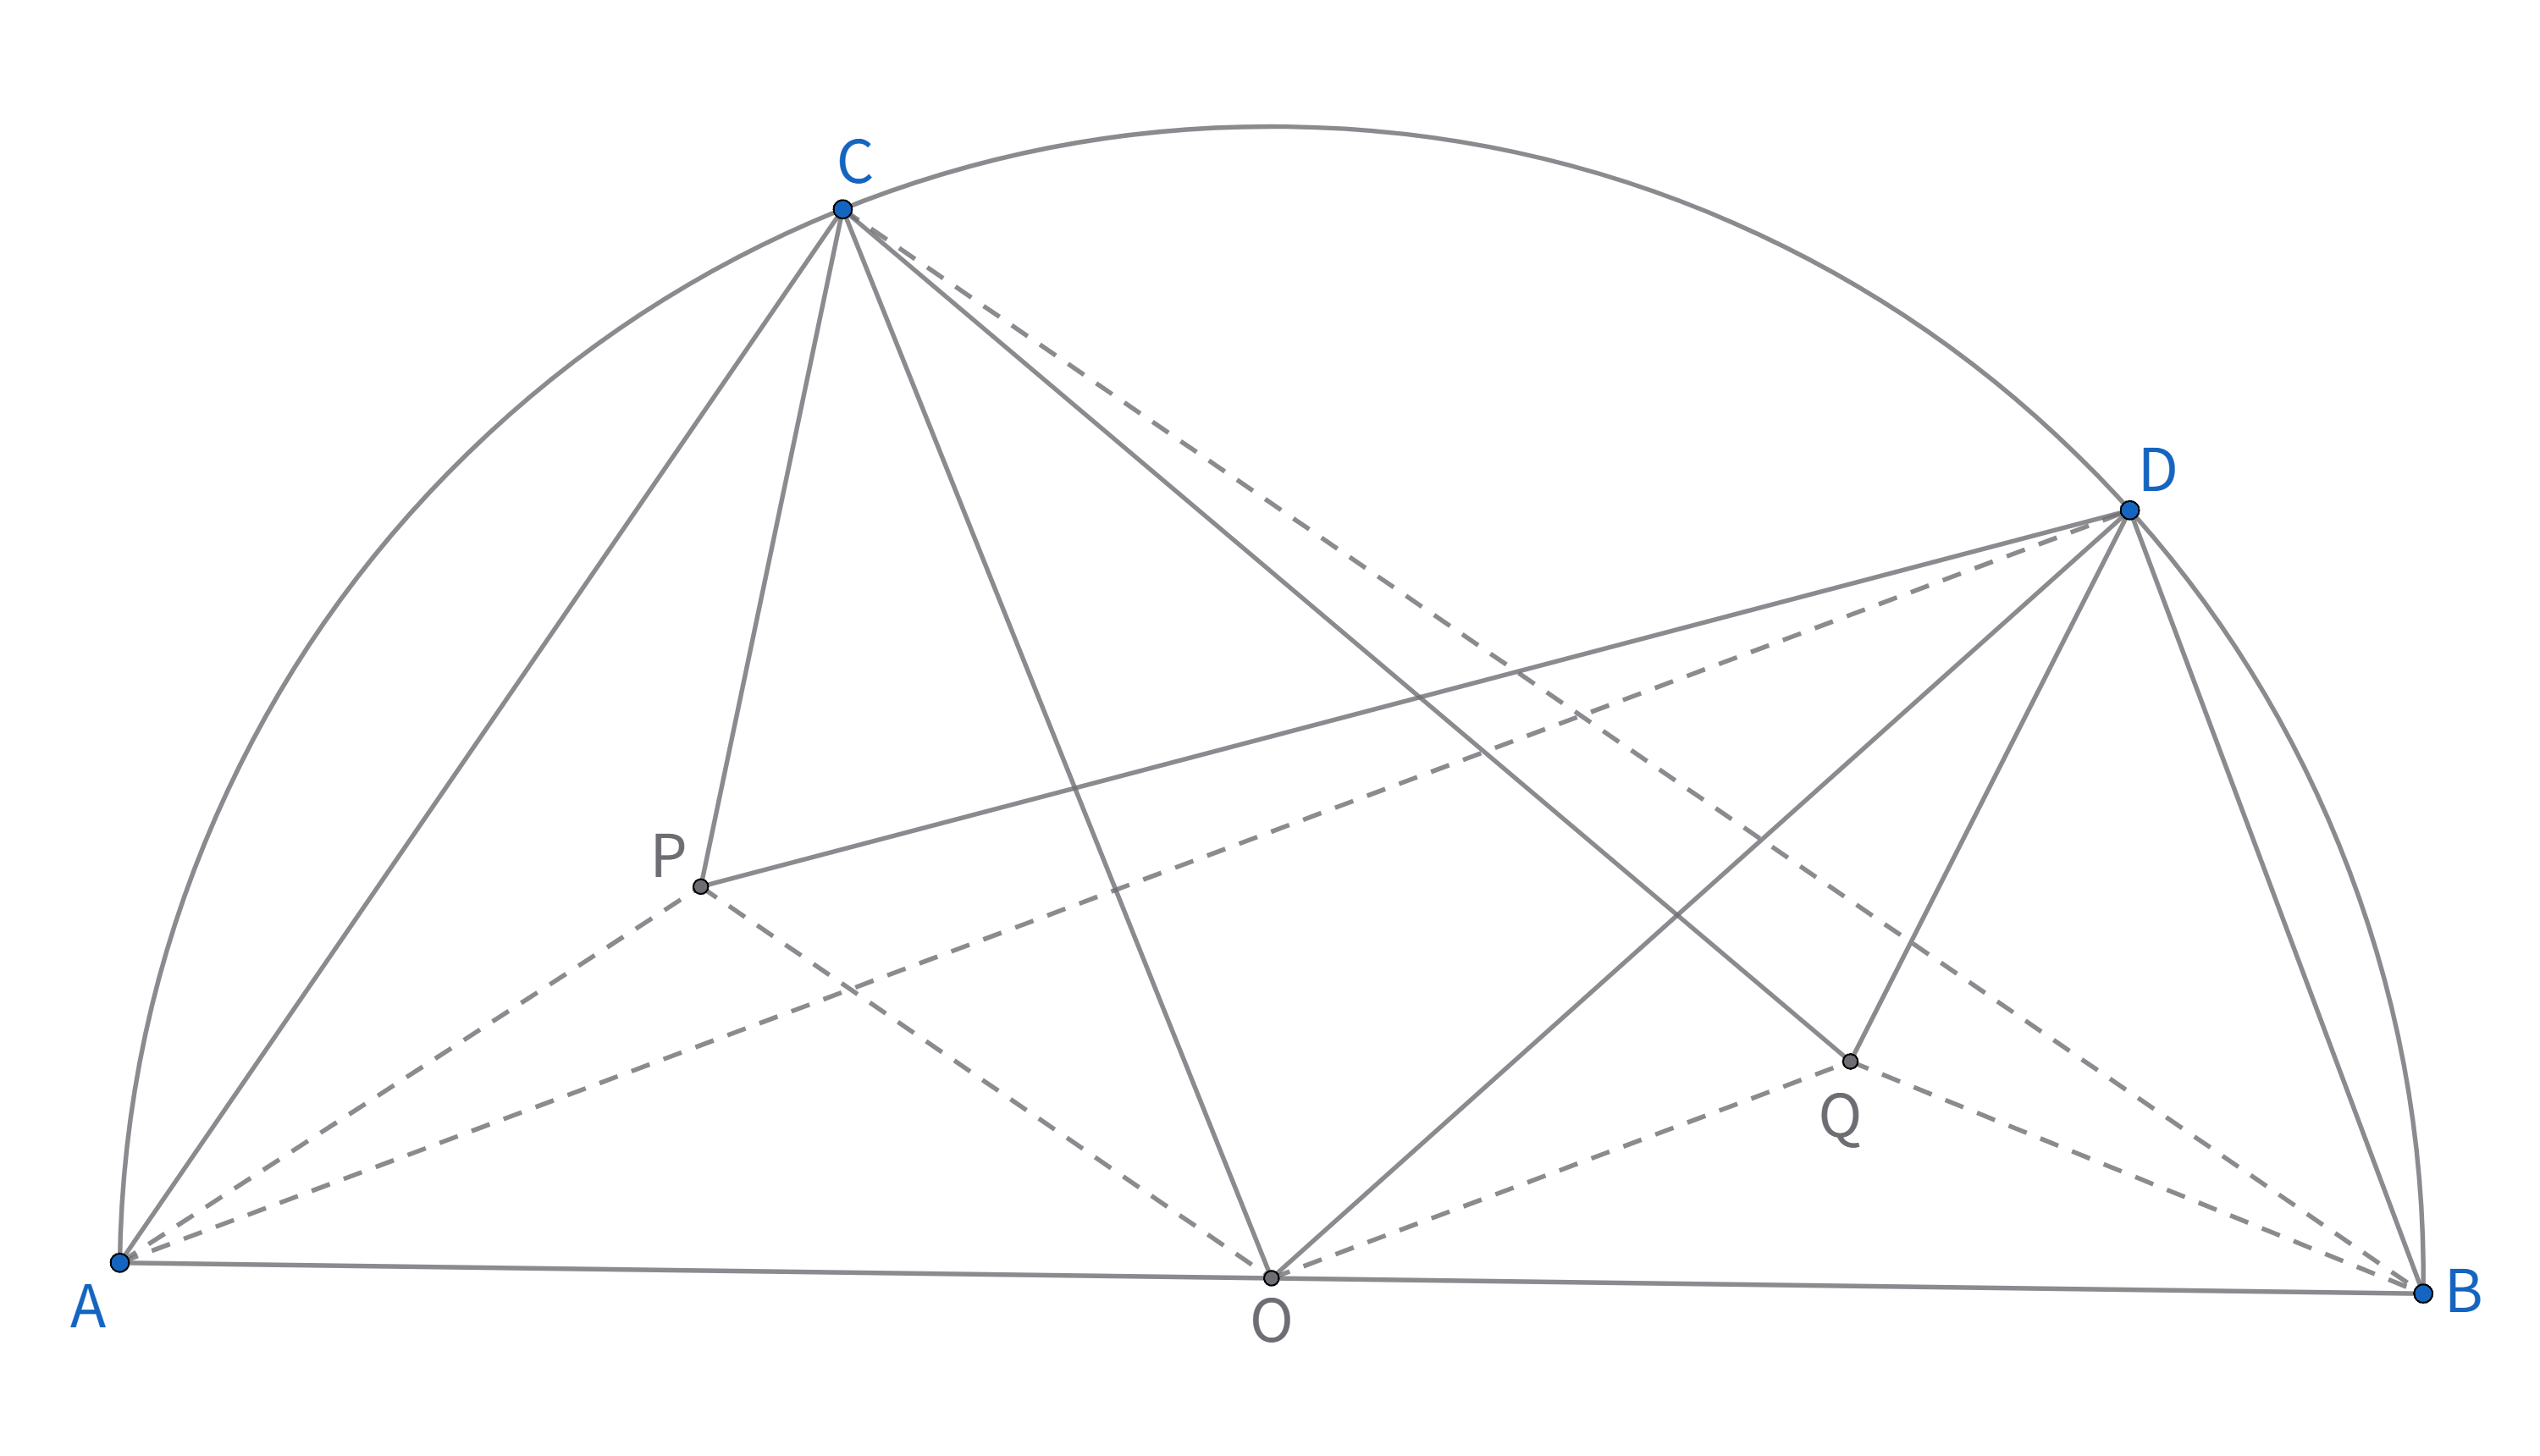
\includegraphics[width=0.5\linewidth]{figures/西部赛14年Q2.png}
\end{figure}


\subsection{Q7}
平面上,点 $O$ 是正三角形 $ABC$ 的中心,点 $P$、$Q$ 满足 $\overrightarrow{OQ} = 2\overrightarrow{PO}$。
证明:
$$
|PA| + |PB| + |PC| \leq |QA| + |QB| + |QC|。
$$
\begin{figure}[htbp]
    \centering
    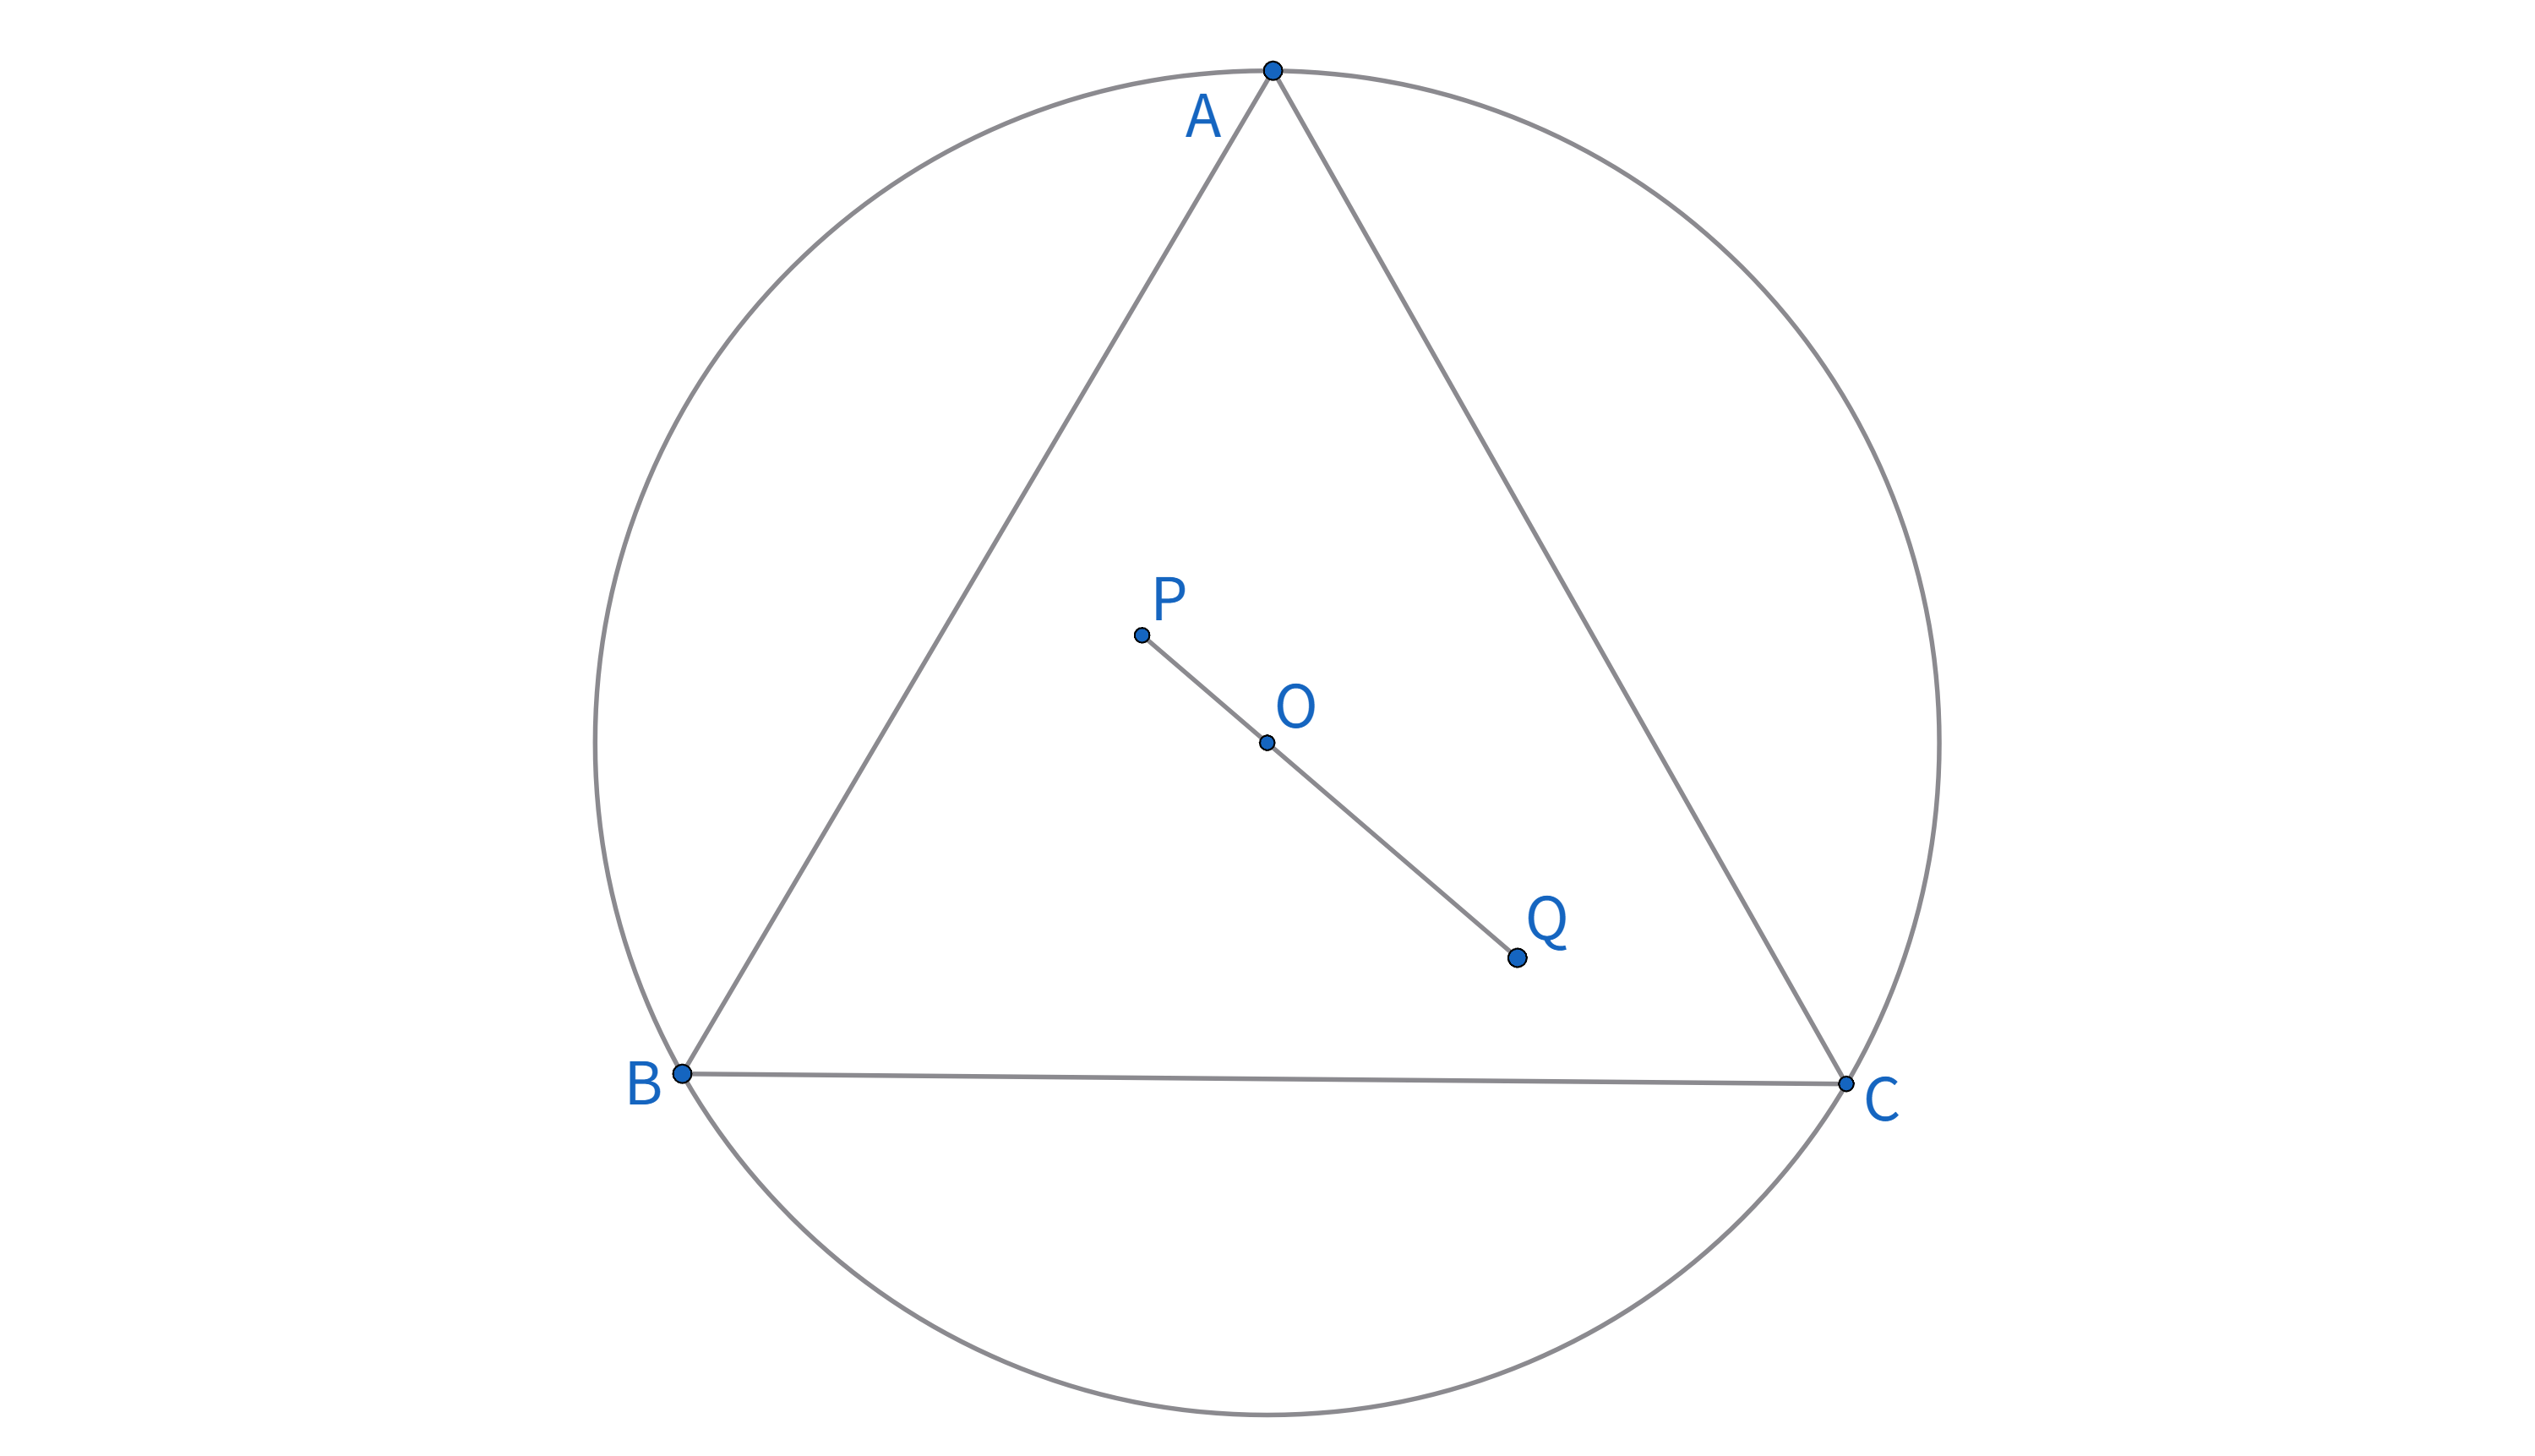
\includegraphics[width=0.7\linewidth]{figures/西部赛14年Q7.png}
\end{figure}


%-------------------------------------------------------------
\newpage 
\section{2013年}
\subsection{Q3}
在 $\triangle ABC$ 中,点 $B_2$ 是 $AC$ 边上旁切圆圆心 $B_1$ 关于 $AC$ 中点的对称点,点 $C_2$ 是 $AB$ 边上旁切圆圆心 $C_1$ 关于 $AB$ 中点的对称点,$BC$ 边上旁切圆切 $BC$ 边于点 $D$。求证:$AD \perp B_2C_2$。
\begin{figure}[htbp]
    \centering
    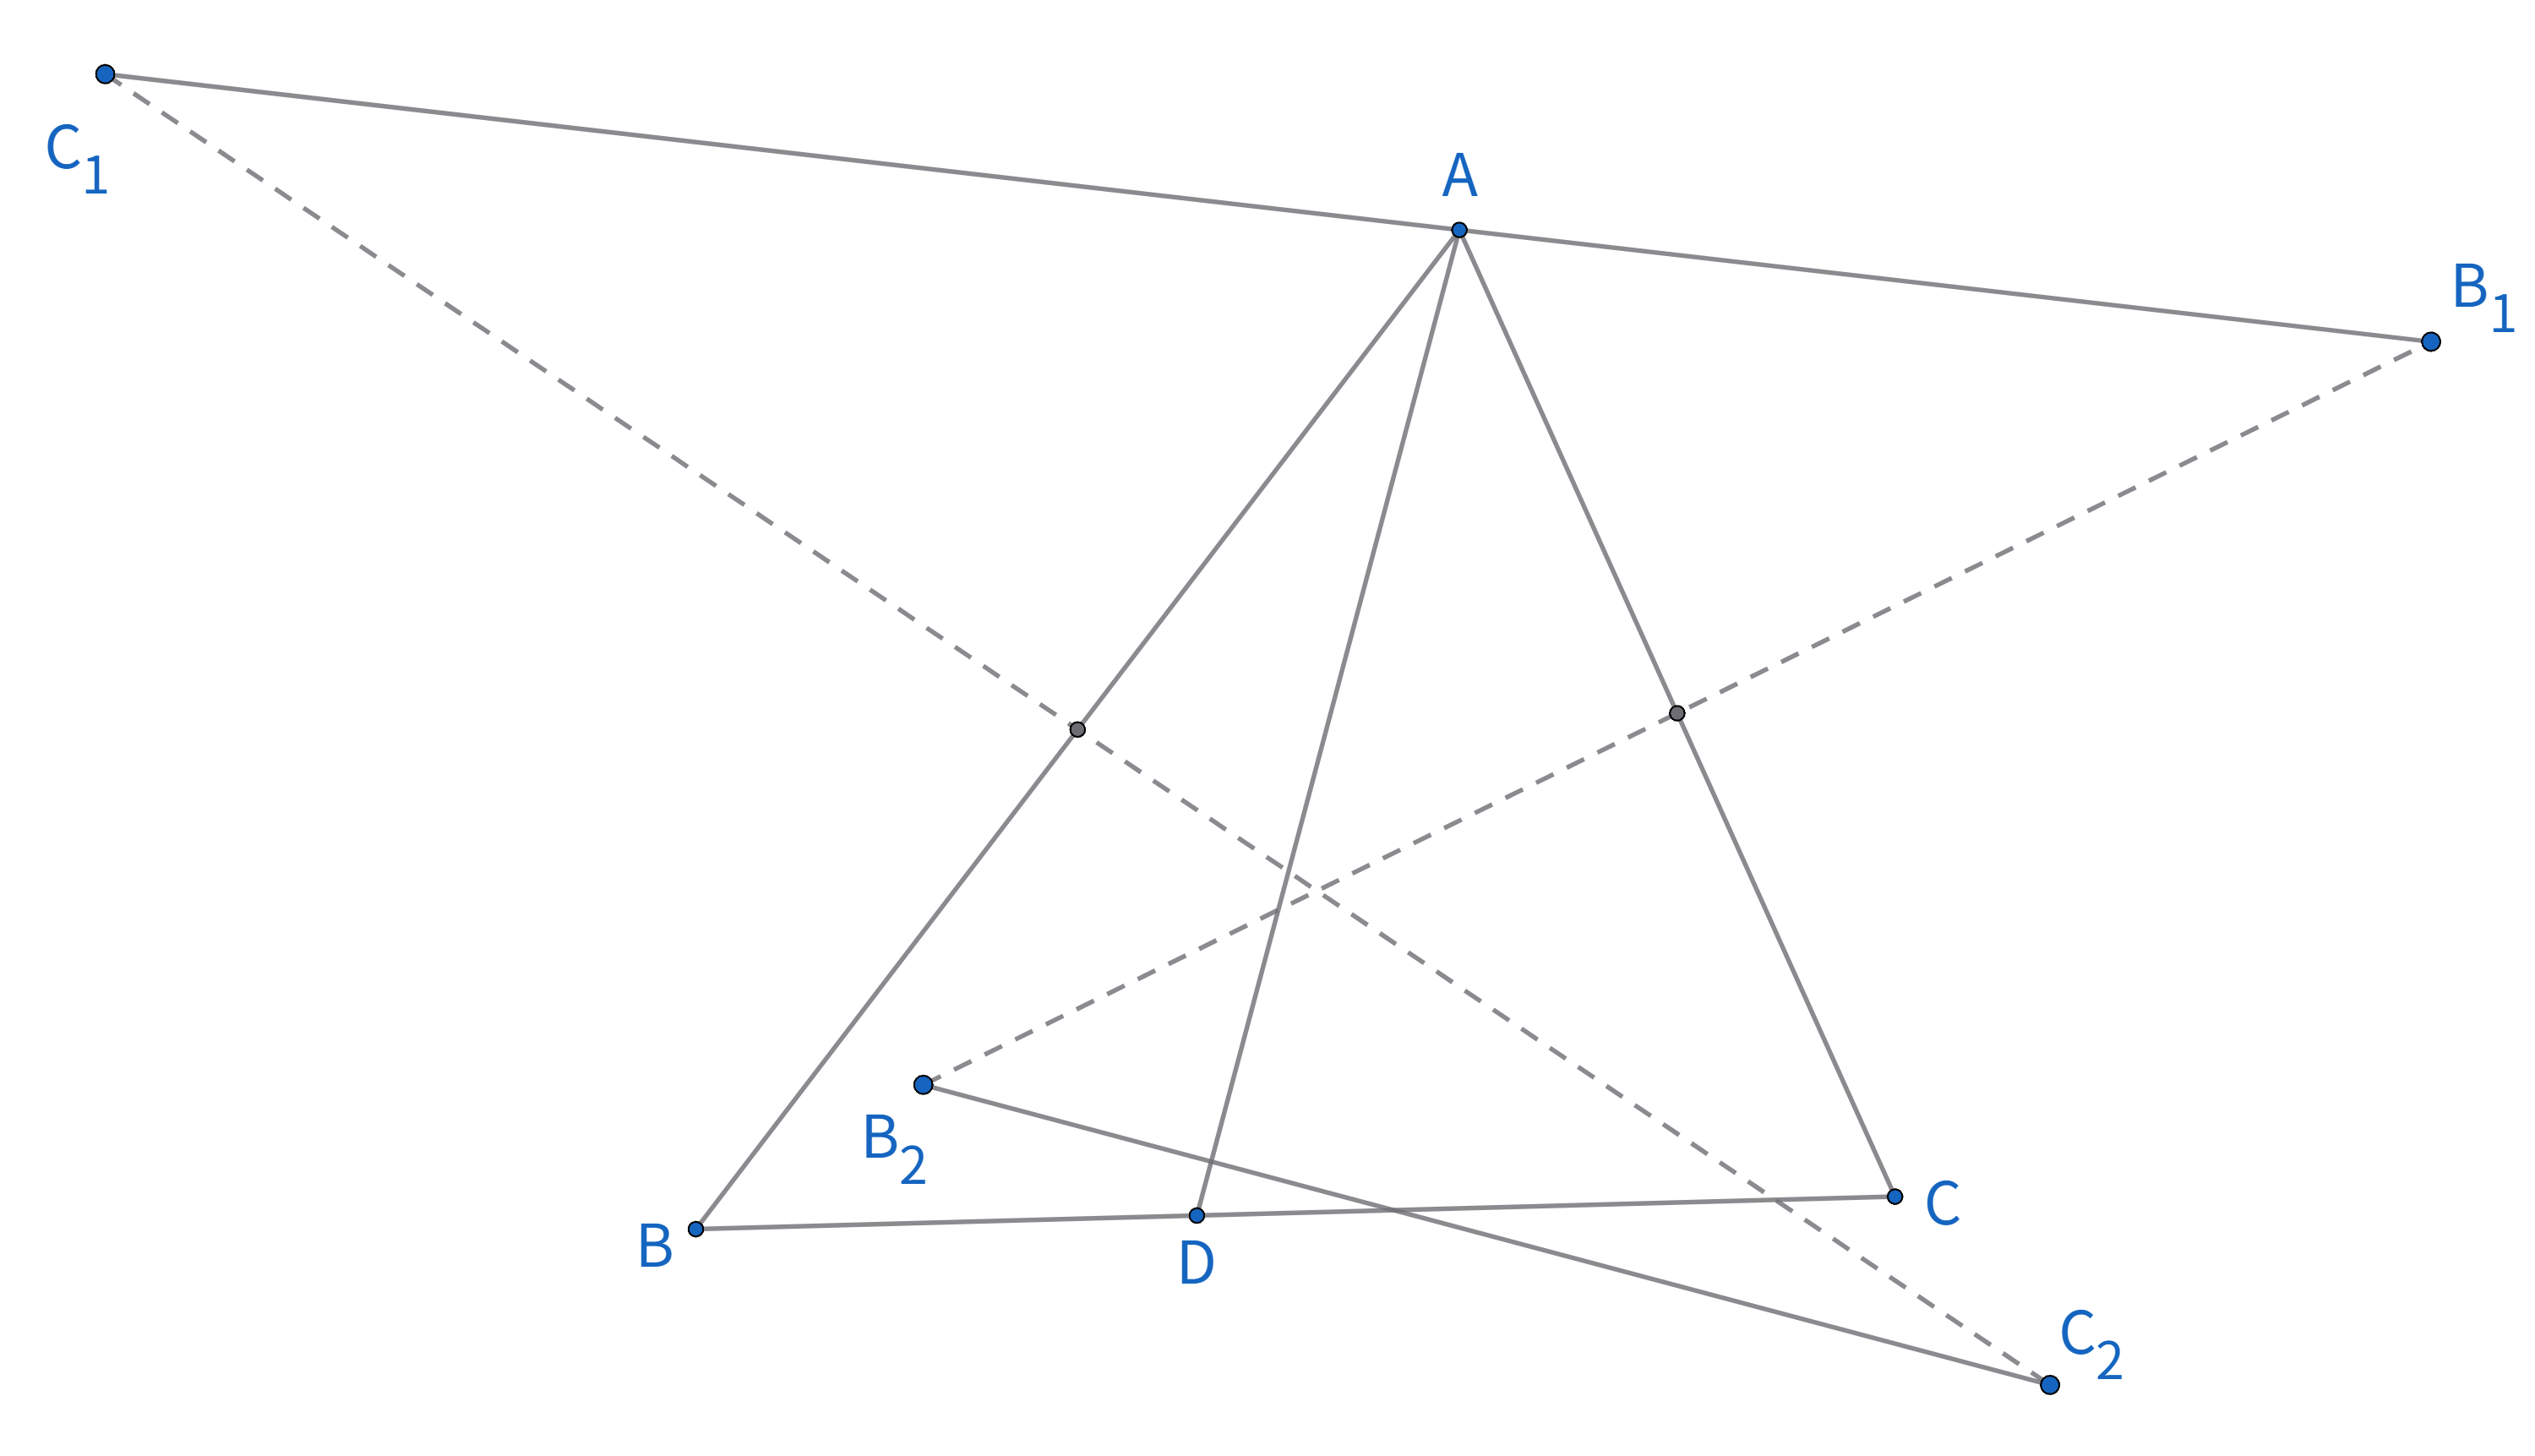
\includegraphics[width=0.7\linewidth]{figures/西部赛13年Q3.png}
\end{figure}


\subsection{Q6}
$PA$、$PB$ 为圆 $O$ 的切线,点 $C$ 在劣弧 $\overset{\frown}{AB}$ 上(不含点 $A$、$B$)。过点 $C$ 作 $PC$ 的垂线 $l$,与 $\angle AOC$ 的平分线交于点 $D$,与 $\angle BOC$ 的平分线交于点 $E$。求证:$CD = CE$。
\begin{figure}[htbp]
    \centering
    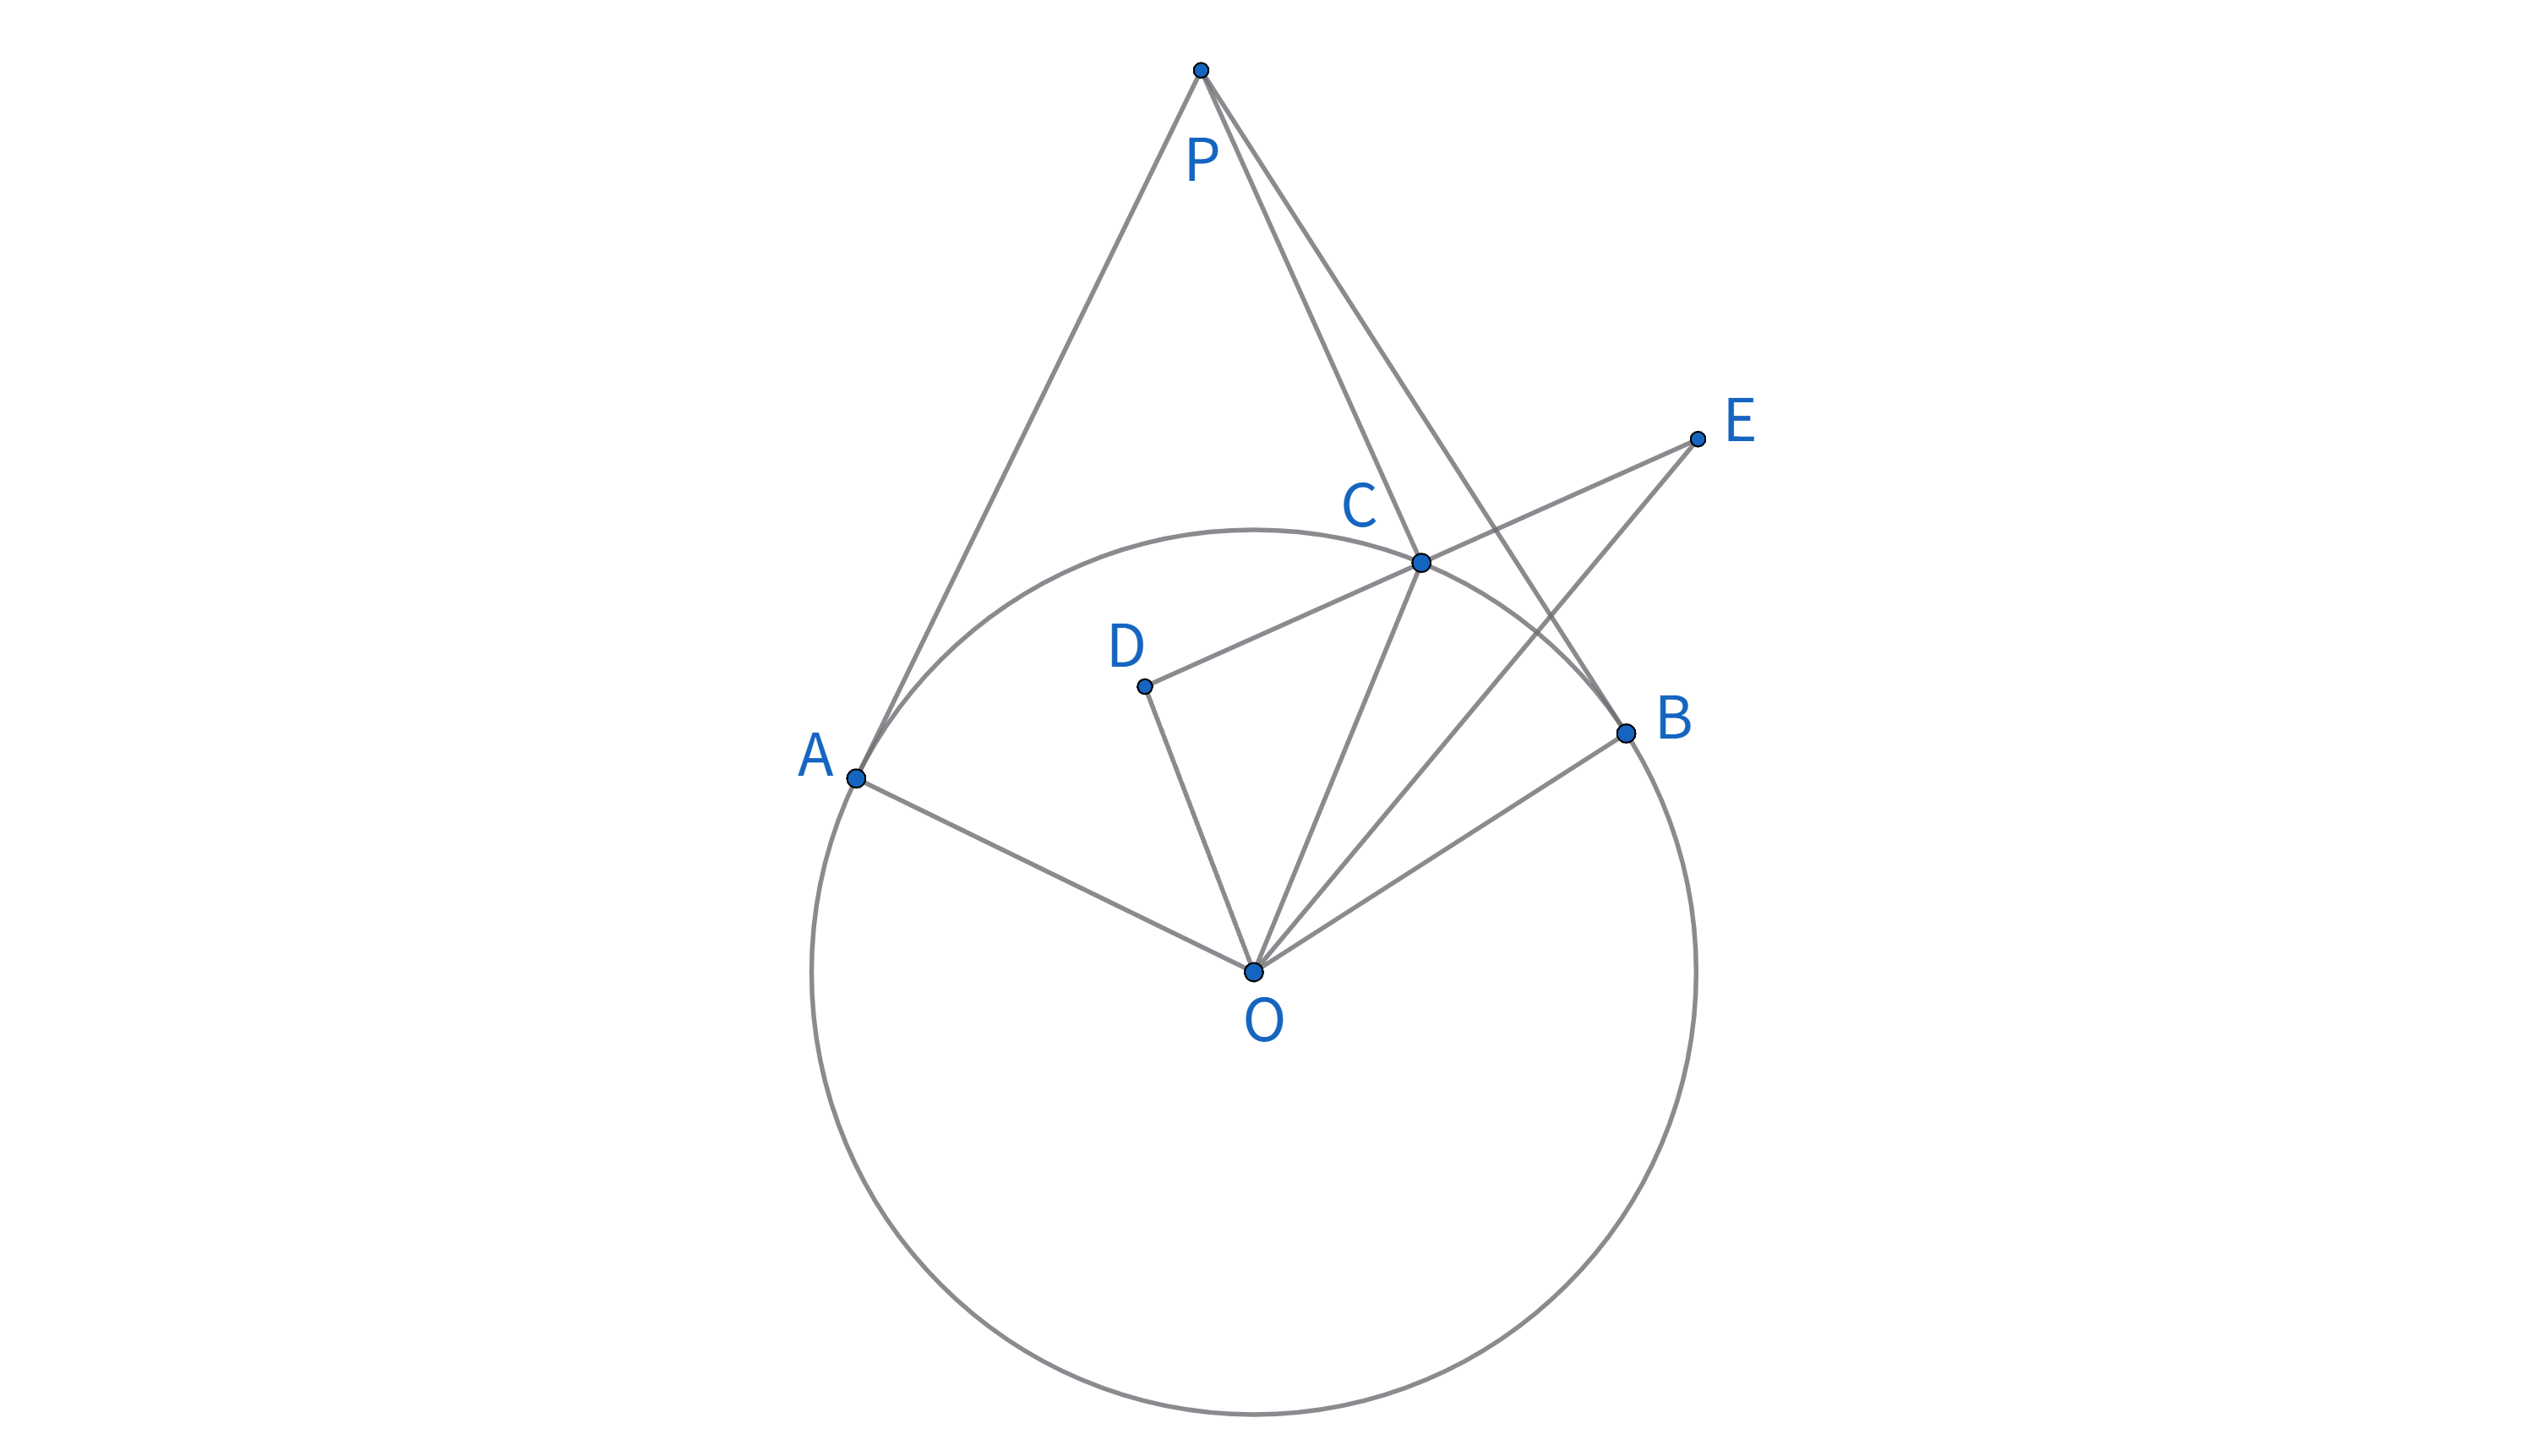
\includegraphics[width=1\linewidth]{figures/西部赛13年Q6.png}
\end{figure}


%-------------------------------------------------------------
\newpage 
\section{2012年}
\subsection{Q4}
已知点 $P$ 为锐角 $\triangle ABC$ 内部任意一点,点 $E$、$F$ 分别为 $P$ 在边 $AC$、$AB$ 上的射影。$BP$、$CP$ 的延长线分别交 $\triangle ABC$ 的外接圆于点 $B_1$、$C_1$,设 $\triangle ABC$ 的外接圆和内切圆的半径分别为 $R$ 和 $r$。求证:$\frac{EF}{B_1C_1} \geq \frac{r}{R}$,并确定等号成立时点 $P$ 的位置。
\begin{figure}[htbp]
    \centering
    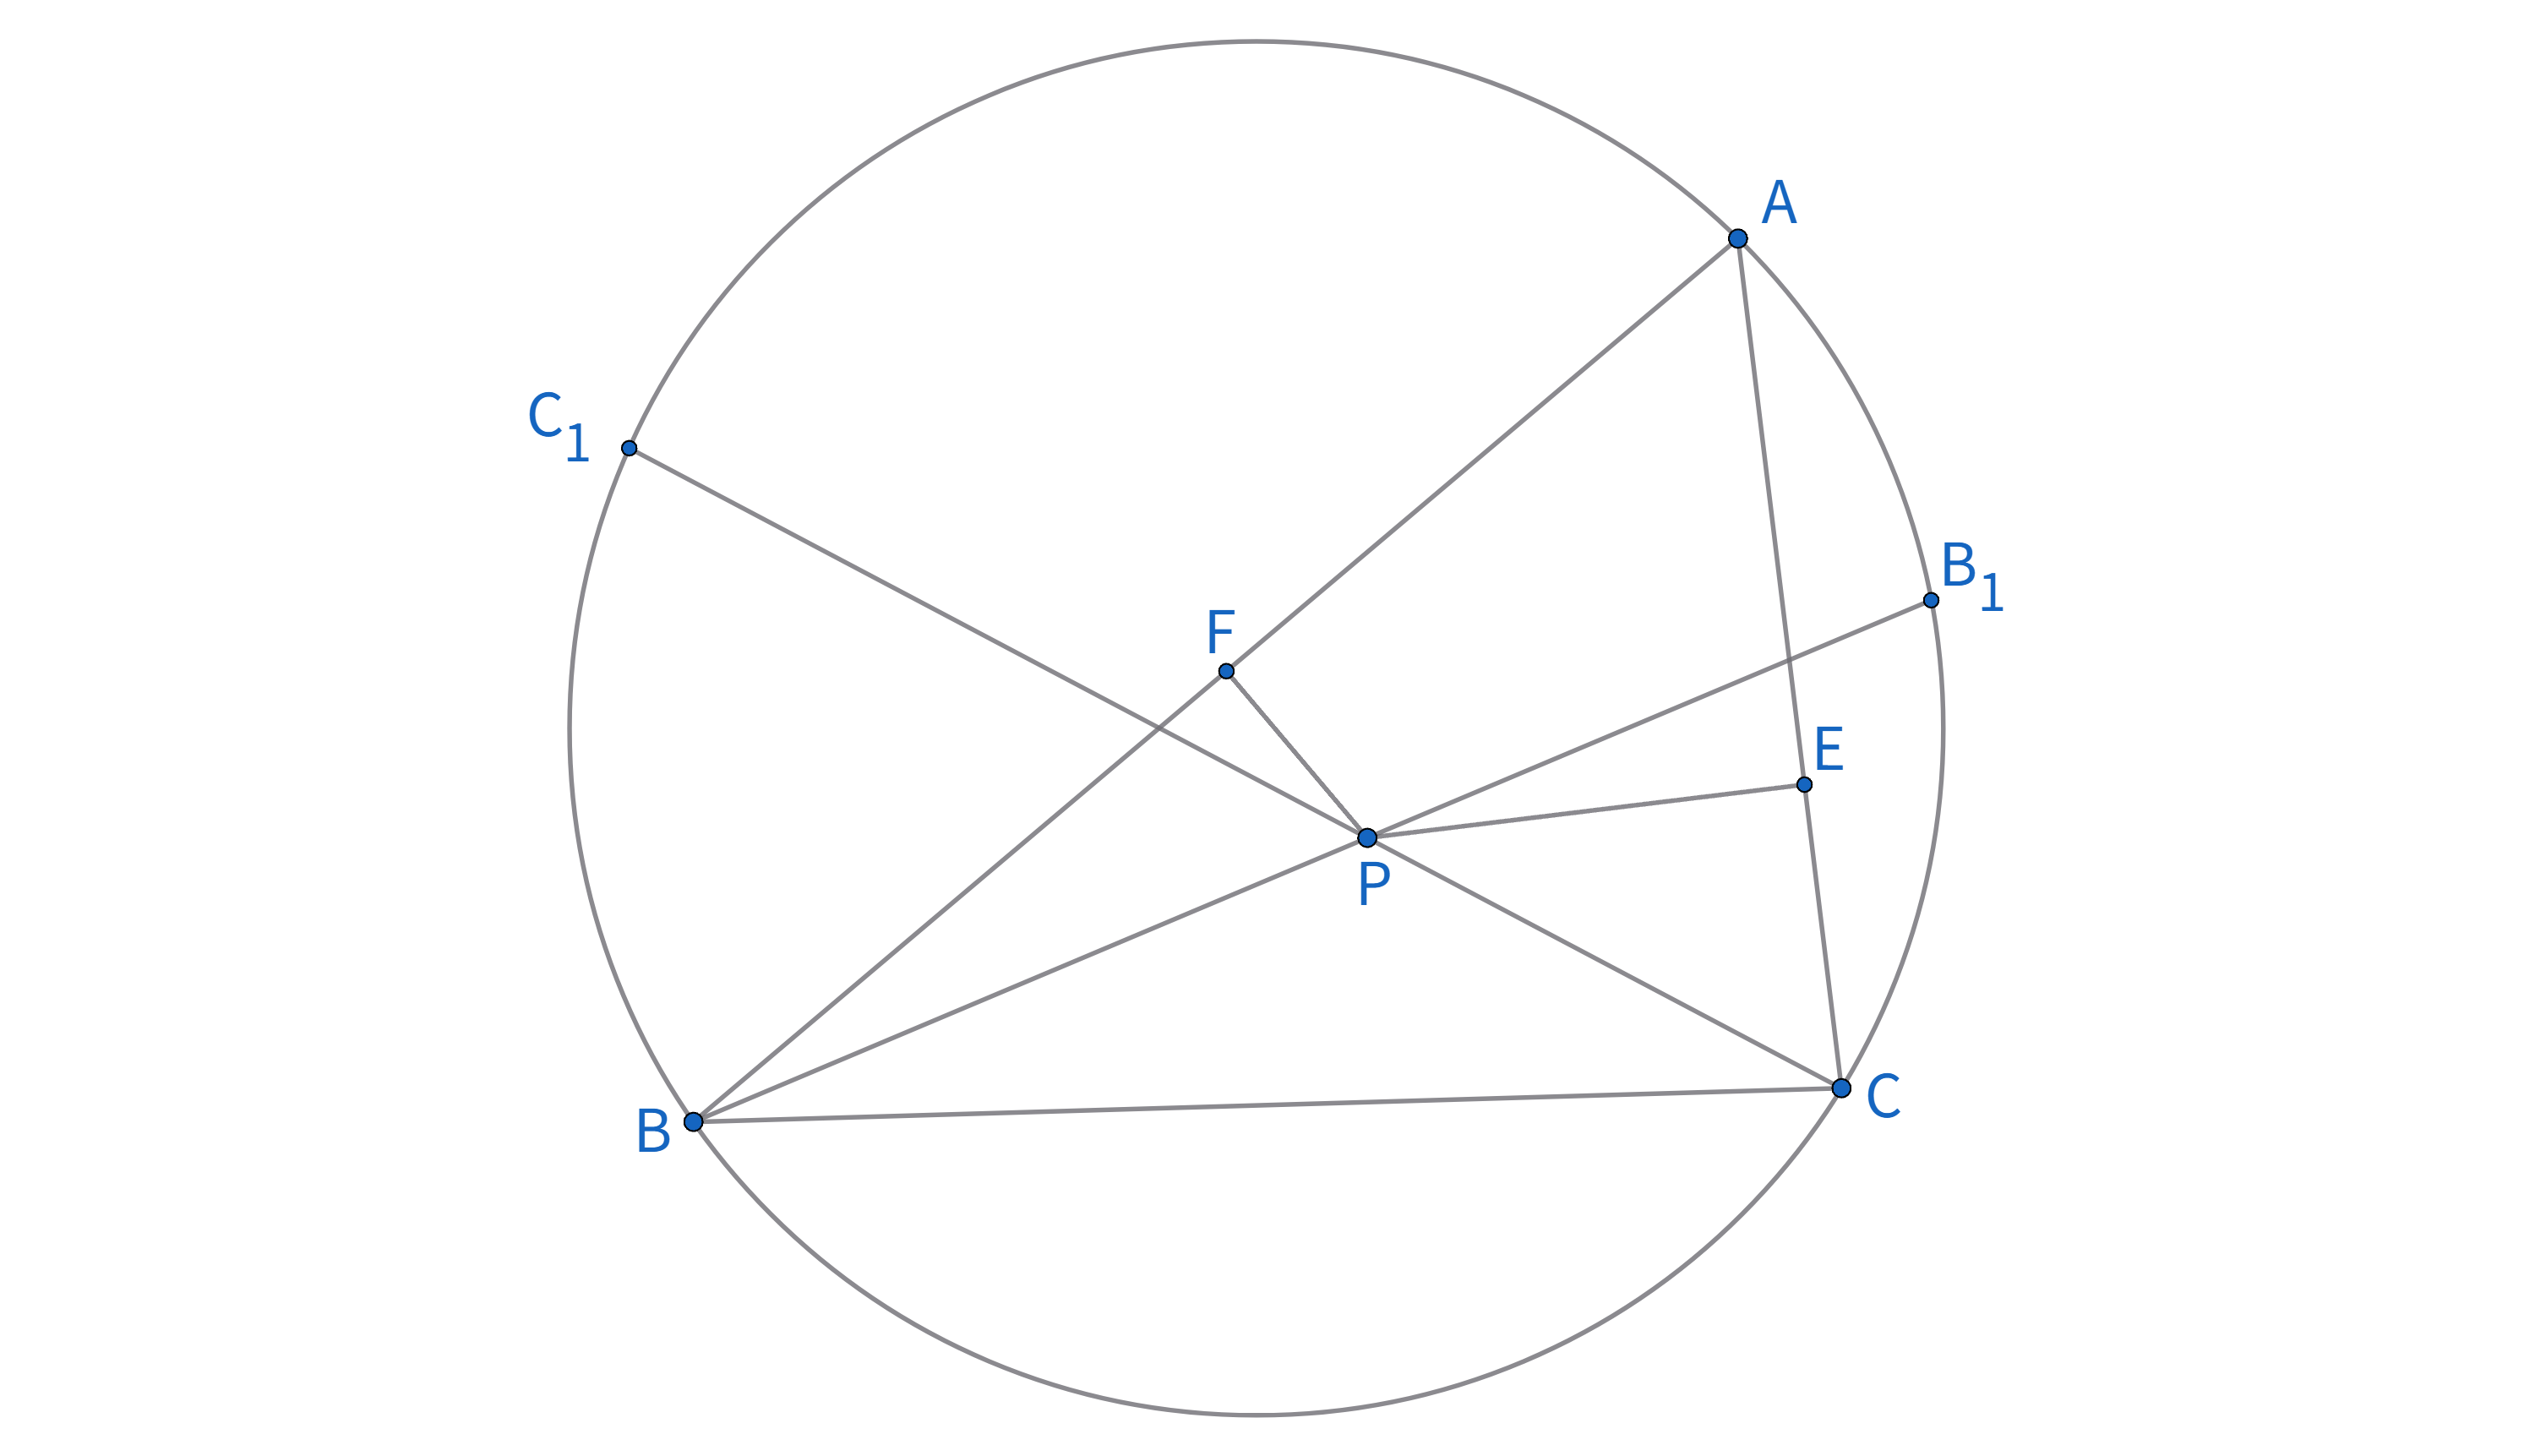
\includegraphics[width=0.8\linewidth]{figures/西部赛12年Q4.png}
\end{figure}


\subsection{Q5}
在锐角 $\triangle ABC$ 中,$H$ 是垂心,$O$ 是外心($A$、$H$、$O$ 三点不共线),点 $D$ 是 $A$ 在边 $BC$ 上的射影,线段 $AO$ 的中垂线交直线 $BC$ 于点 $E$。求证:线段 $OH$ 的中点在 $\triangle ADE$ 的外接圆上。
\begin{figure}[htbp]
    \centering
    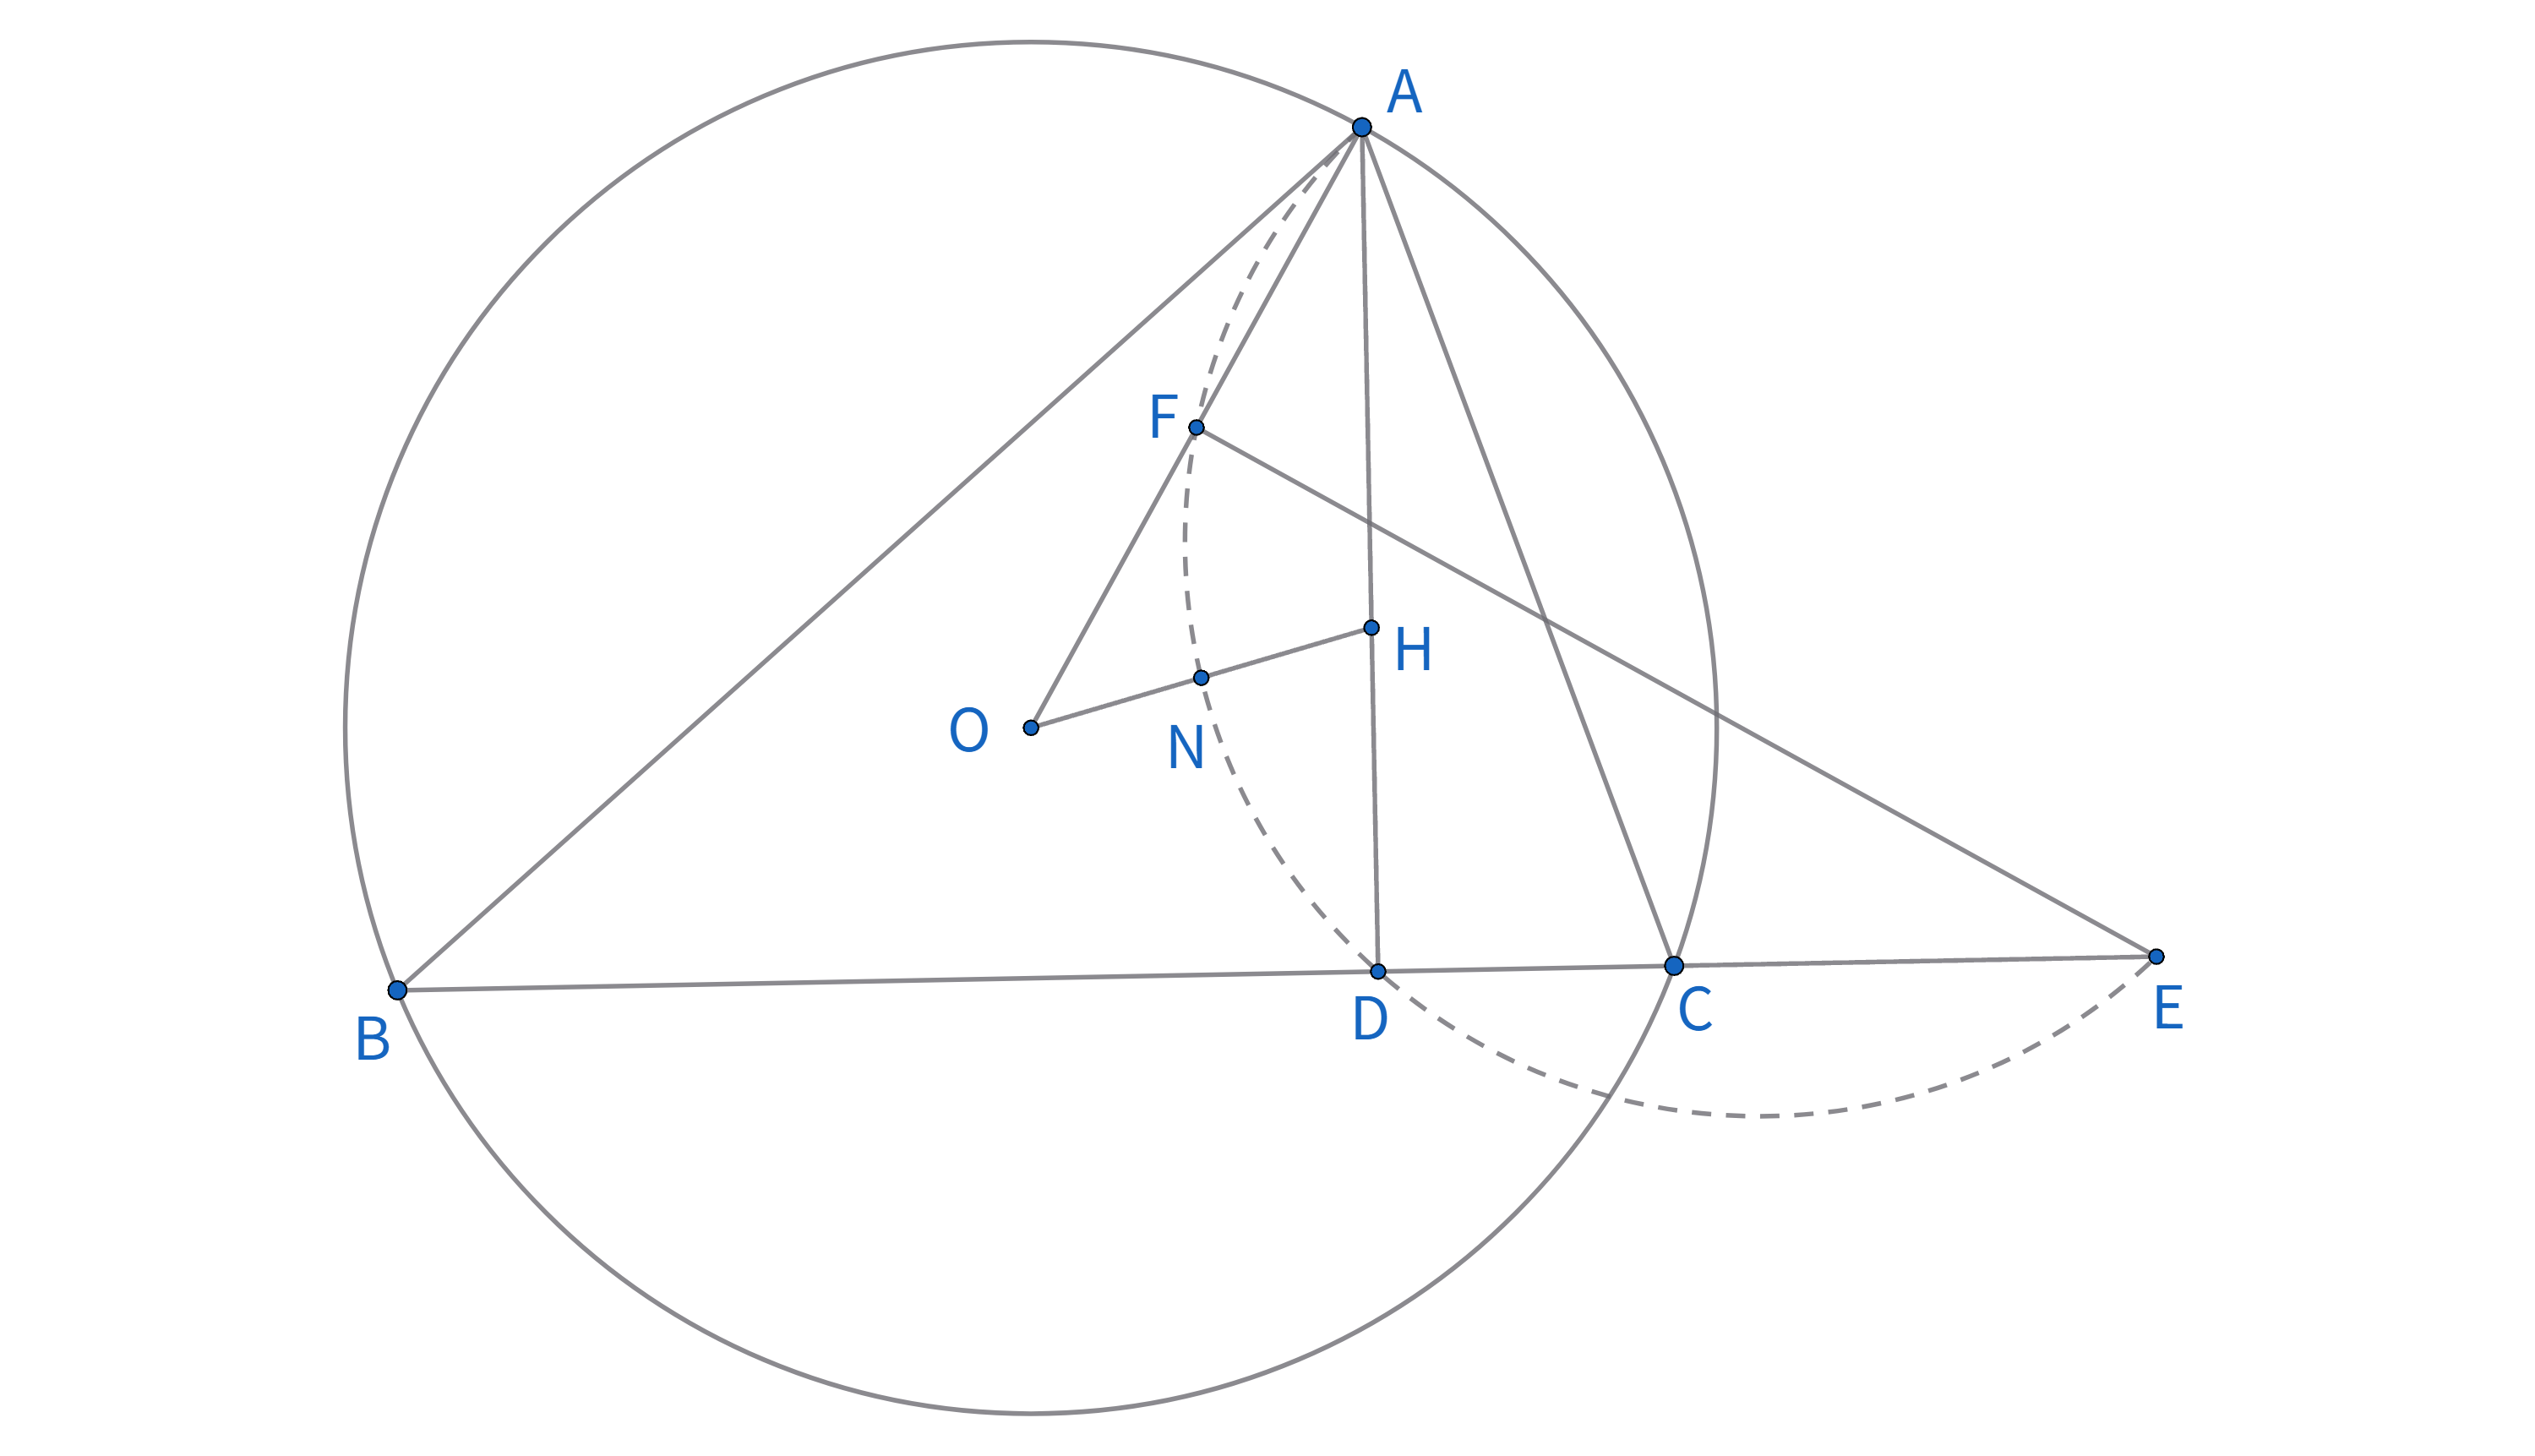
\includegraphics[width=0.8\linewidth]{figures/西部赛12年Q5.png}
\end{figure}



%-------------------------------------------------------------
\newpage 
\section{2011年}
\subsection{Q4}
线段 $AB$、$CD$ 是 $\odot O$ 中长度不相等的两条弦,$AB$ 与 $CD$ 的交点为 $E$,$\odot I$ 内切 $\odot O$ 于点 $F$,且分别与弦 $AB$、$CD$ 相切于点 $G$、$H$。过点 $O$ 的直线 $l$ 分别交 $AB$、$CD$ 于点 $P$、$Q$,使得 $EP = EQ$。直线 $EF$ 与直线 $l$ 交于点 $M$,求证:过点 $M$ 且与 $AB$ 平行的直线是 $\odot O$ 的切线。
\begin{figure}[htbp]
    \centering
    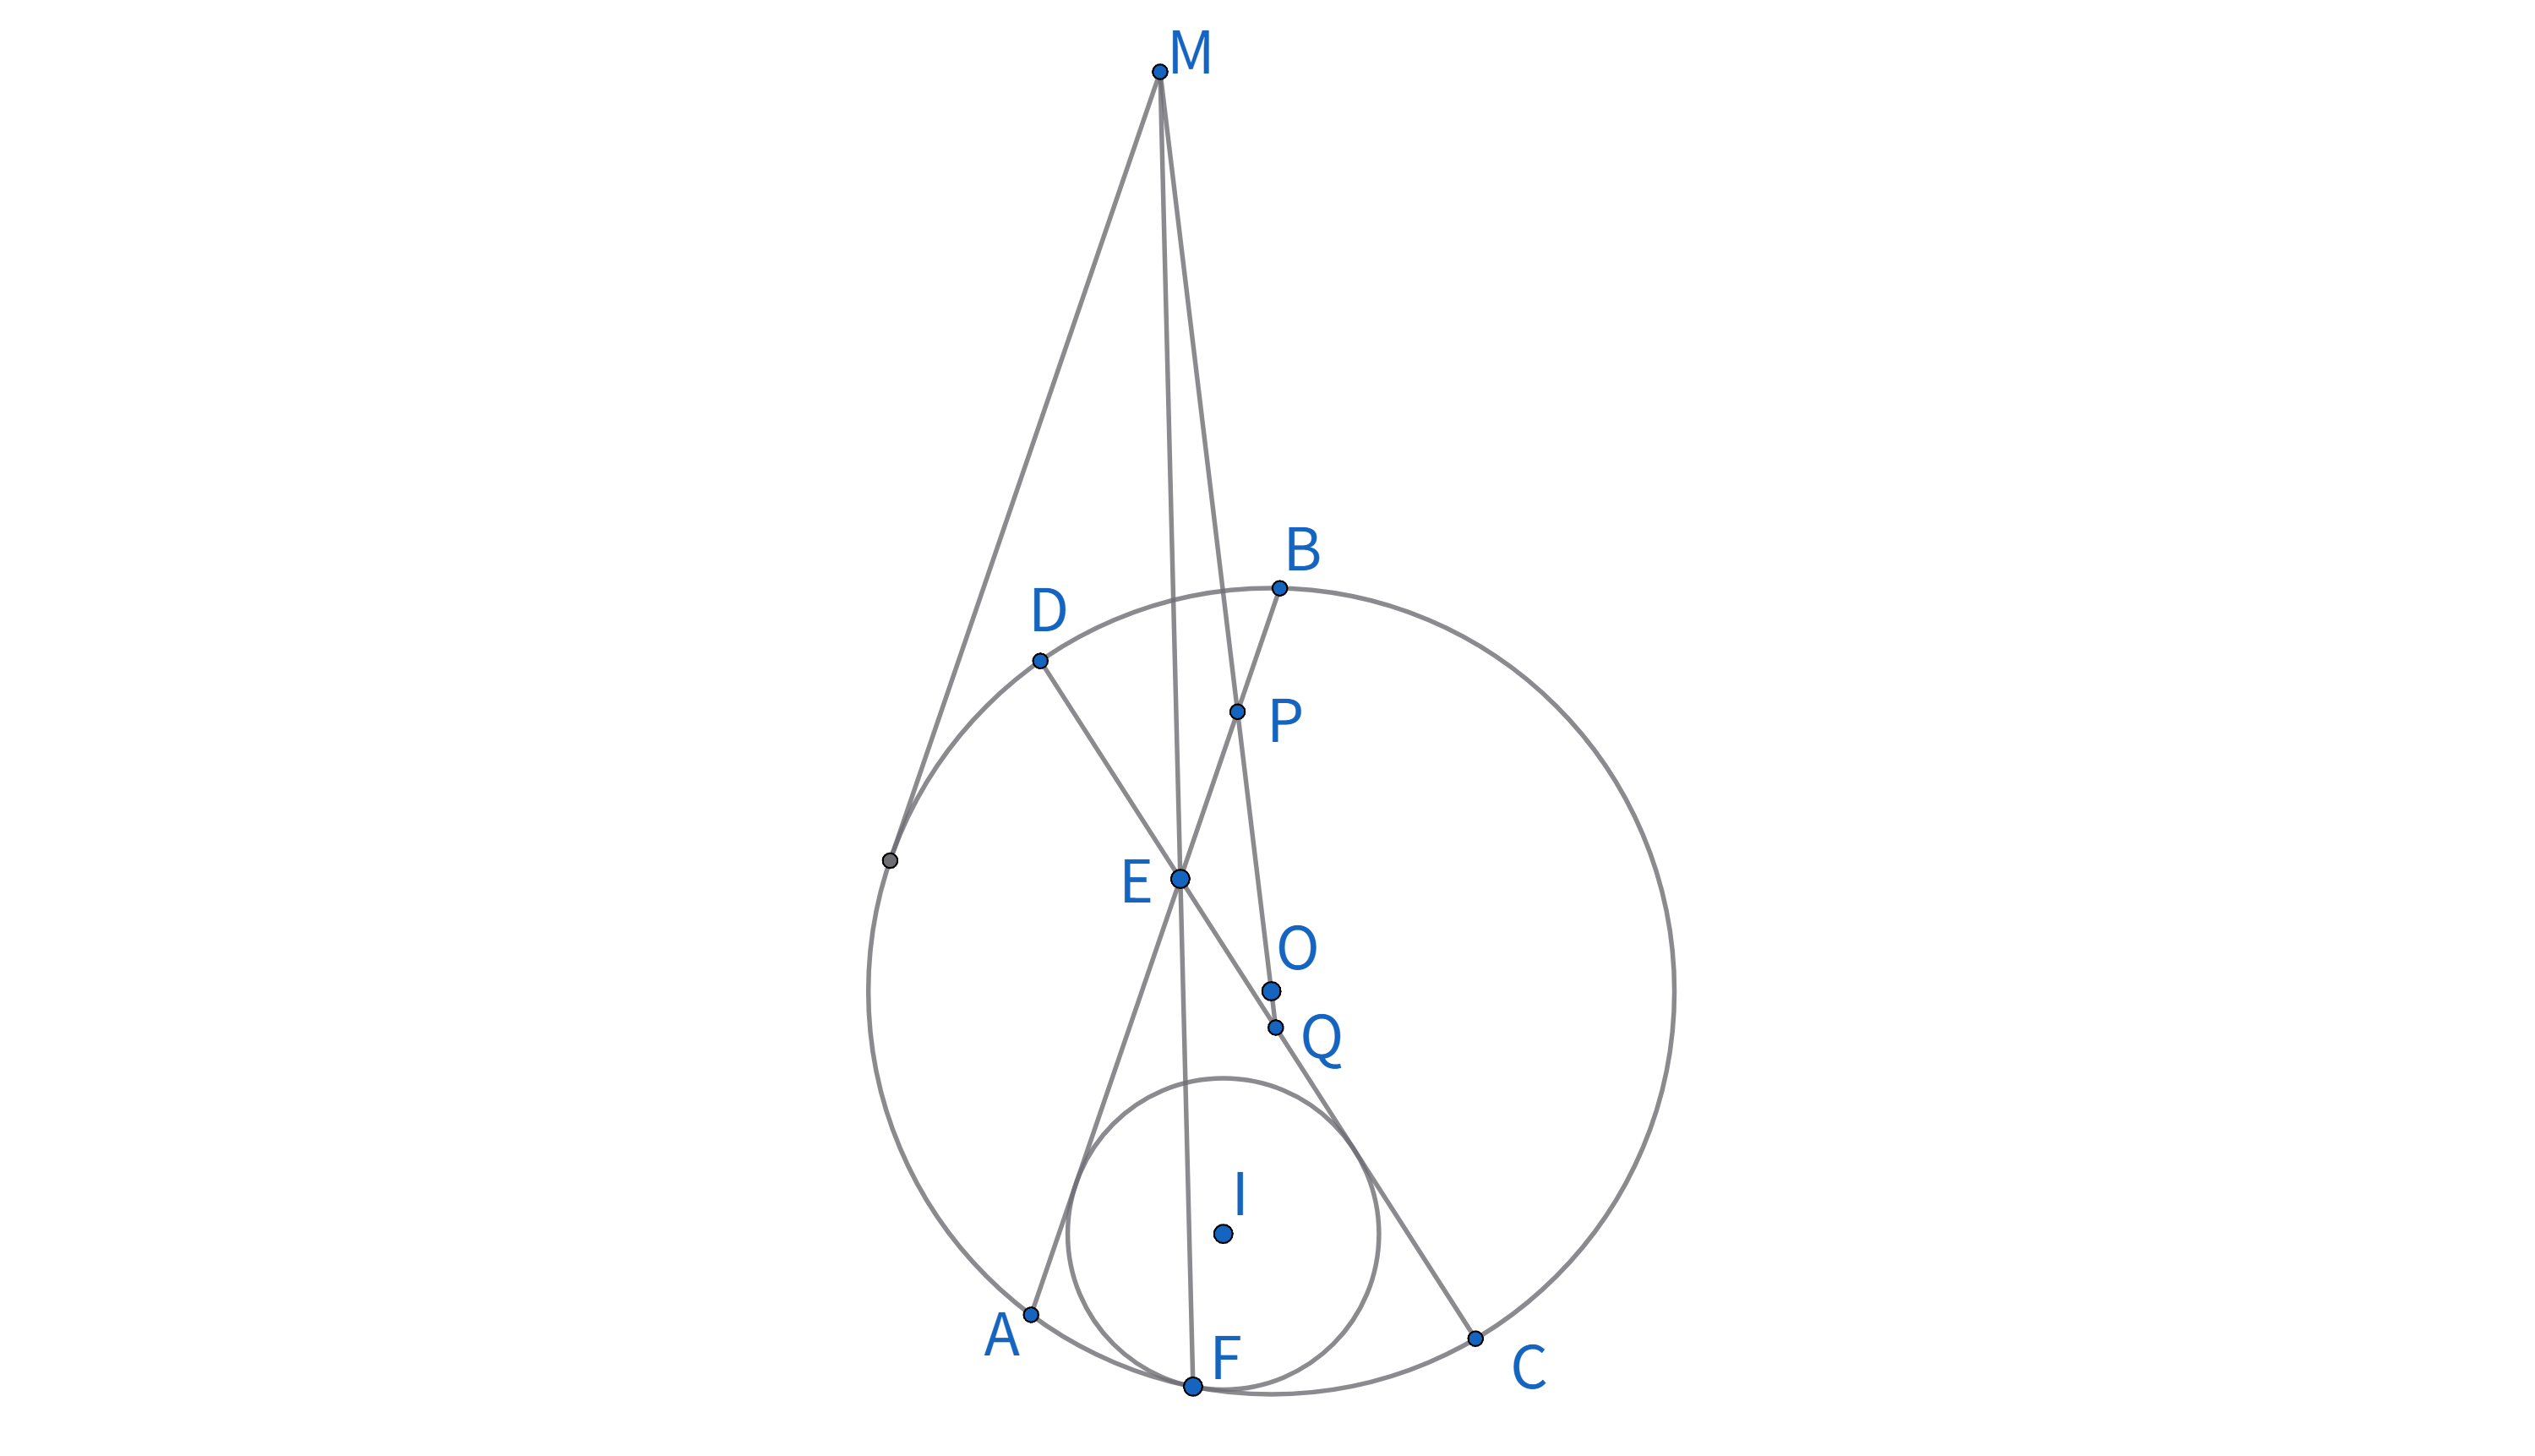
\includegraphics[width=0.8\linewidth]{figures/西部赛11年Q4.png}
\end{figure}

\subsection{Q7}
在 $\triangle ABC$ 中,$AB > AC$,内切圆 $\odot I$ 与边 $BC$、$CA$、$AB$ 分别相切于点 $D$、$E$、$F$,$M$ 是边 $BC$ 的中点,$AH \perp BC$ 于点 $H$。$\angle BAC$ 的平分线 $AI$ 分别与直线 $DE$、$DF$ 交于点 $K$、$L$。求证:$M$、$L$、$H$、$K$ 四点共圆。
\begin{figure}[htbp]
    \centering
    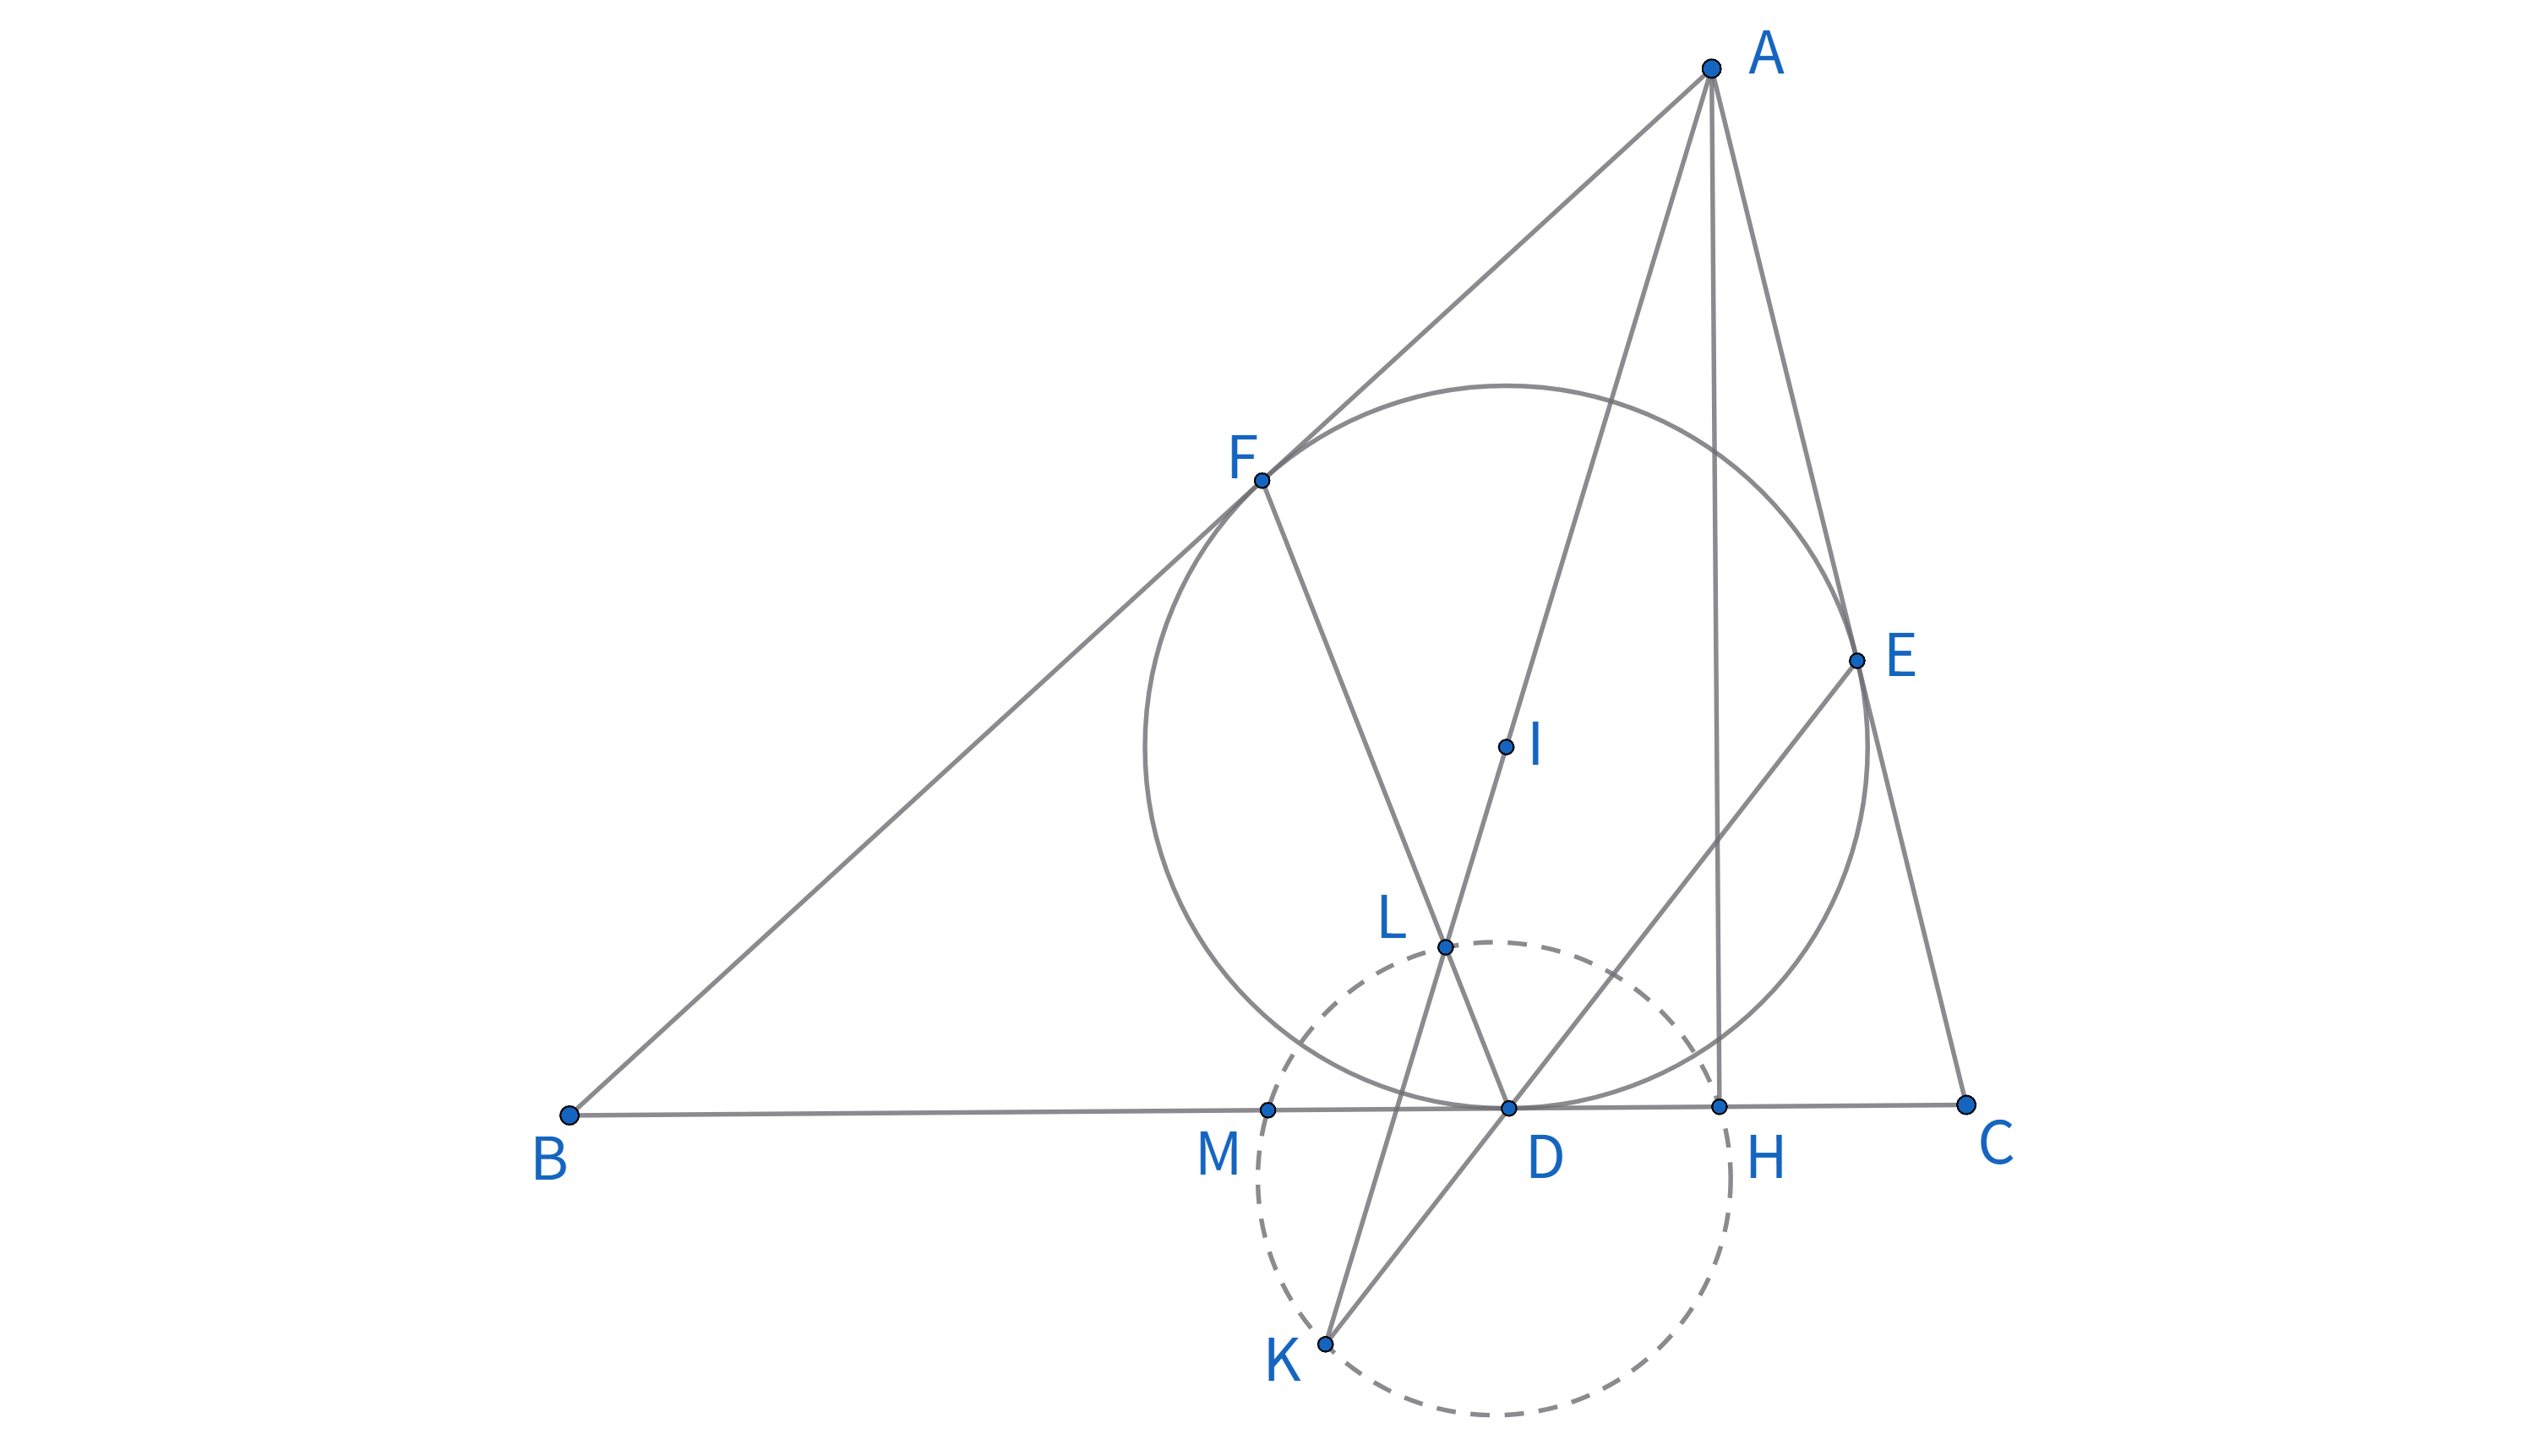
\includegraphics[width=0.7\linewidth]{figures/西部赛11年Q7.png}
\end{figure}


%-------------------------------------------------------------
\newpage
\section{2010年}
\subsection{Q2}
$AB$ 是 $\odot O$ 的直径,$C$、$D$ 是圆周上异于 $A$、$B$ 且在 $AB$ 同侧的两点,分别过点 $C$、$D$ 作圆的切线,它们相交于点 $E$,线段 $AD$ 与 $BC$ 的交点为 $F$,直线 $EF$ 与 $AB$ 相交于点 $M$,求证:$E$、$C$、$M$、$D$ 四点共圆。
\begin{figure}[htbp]
    \centering
    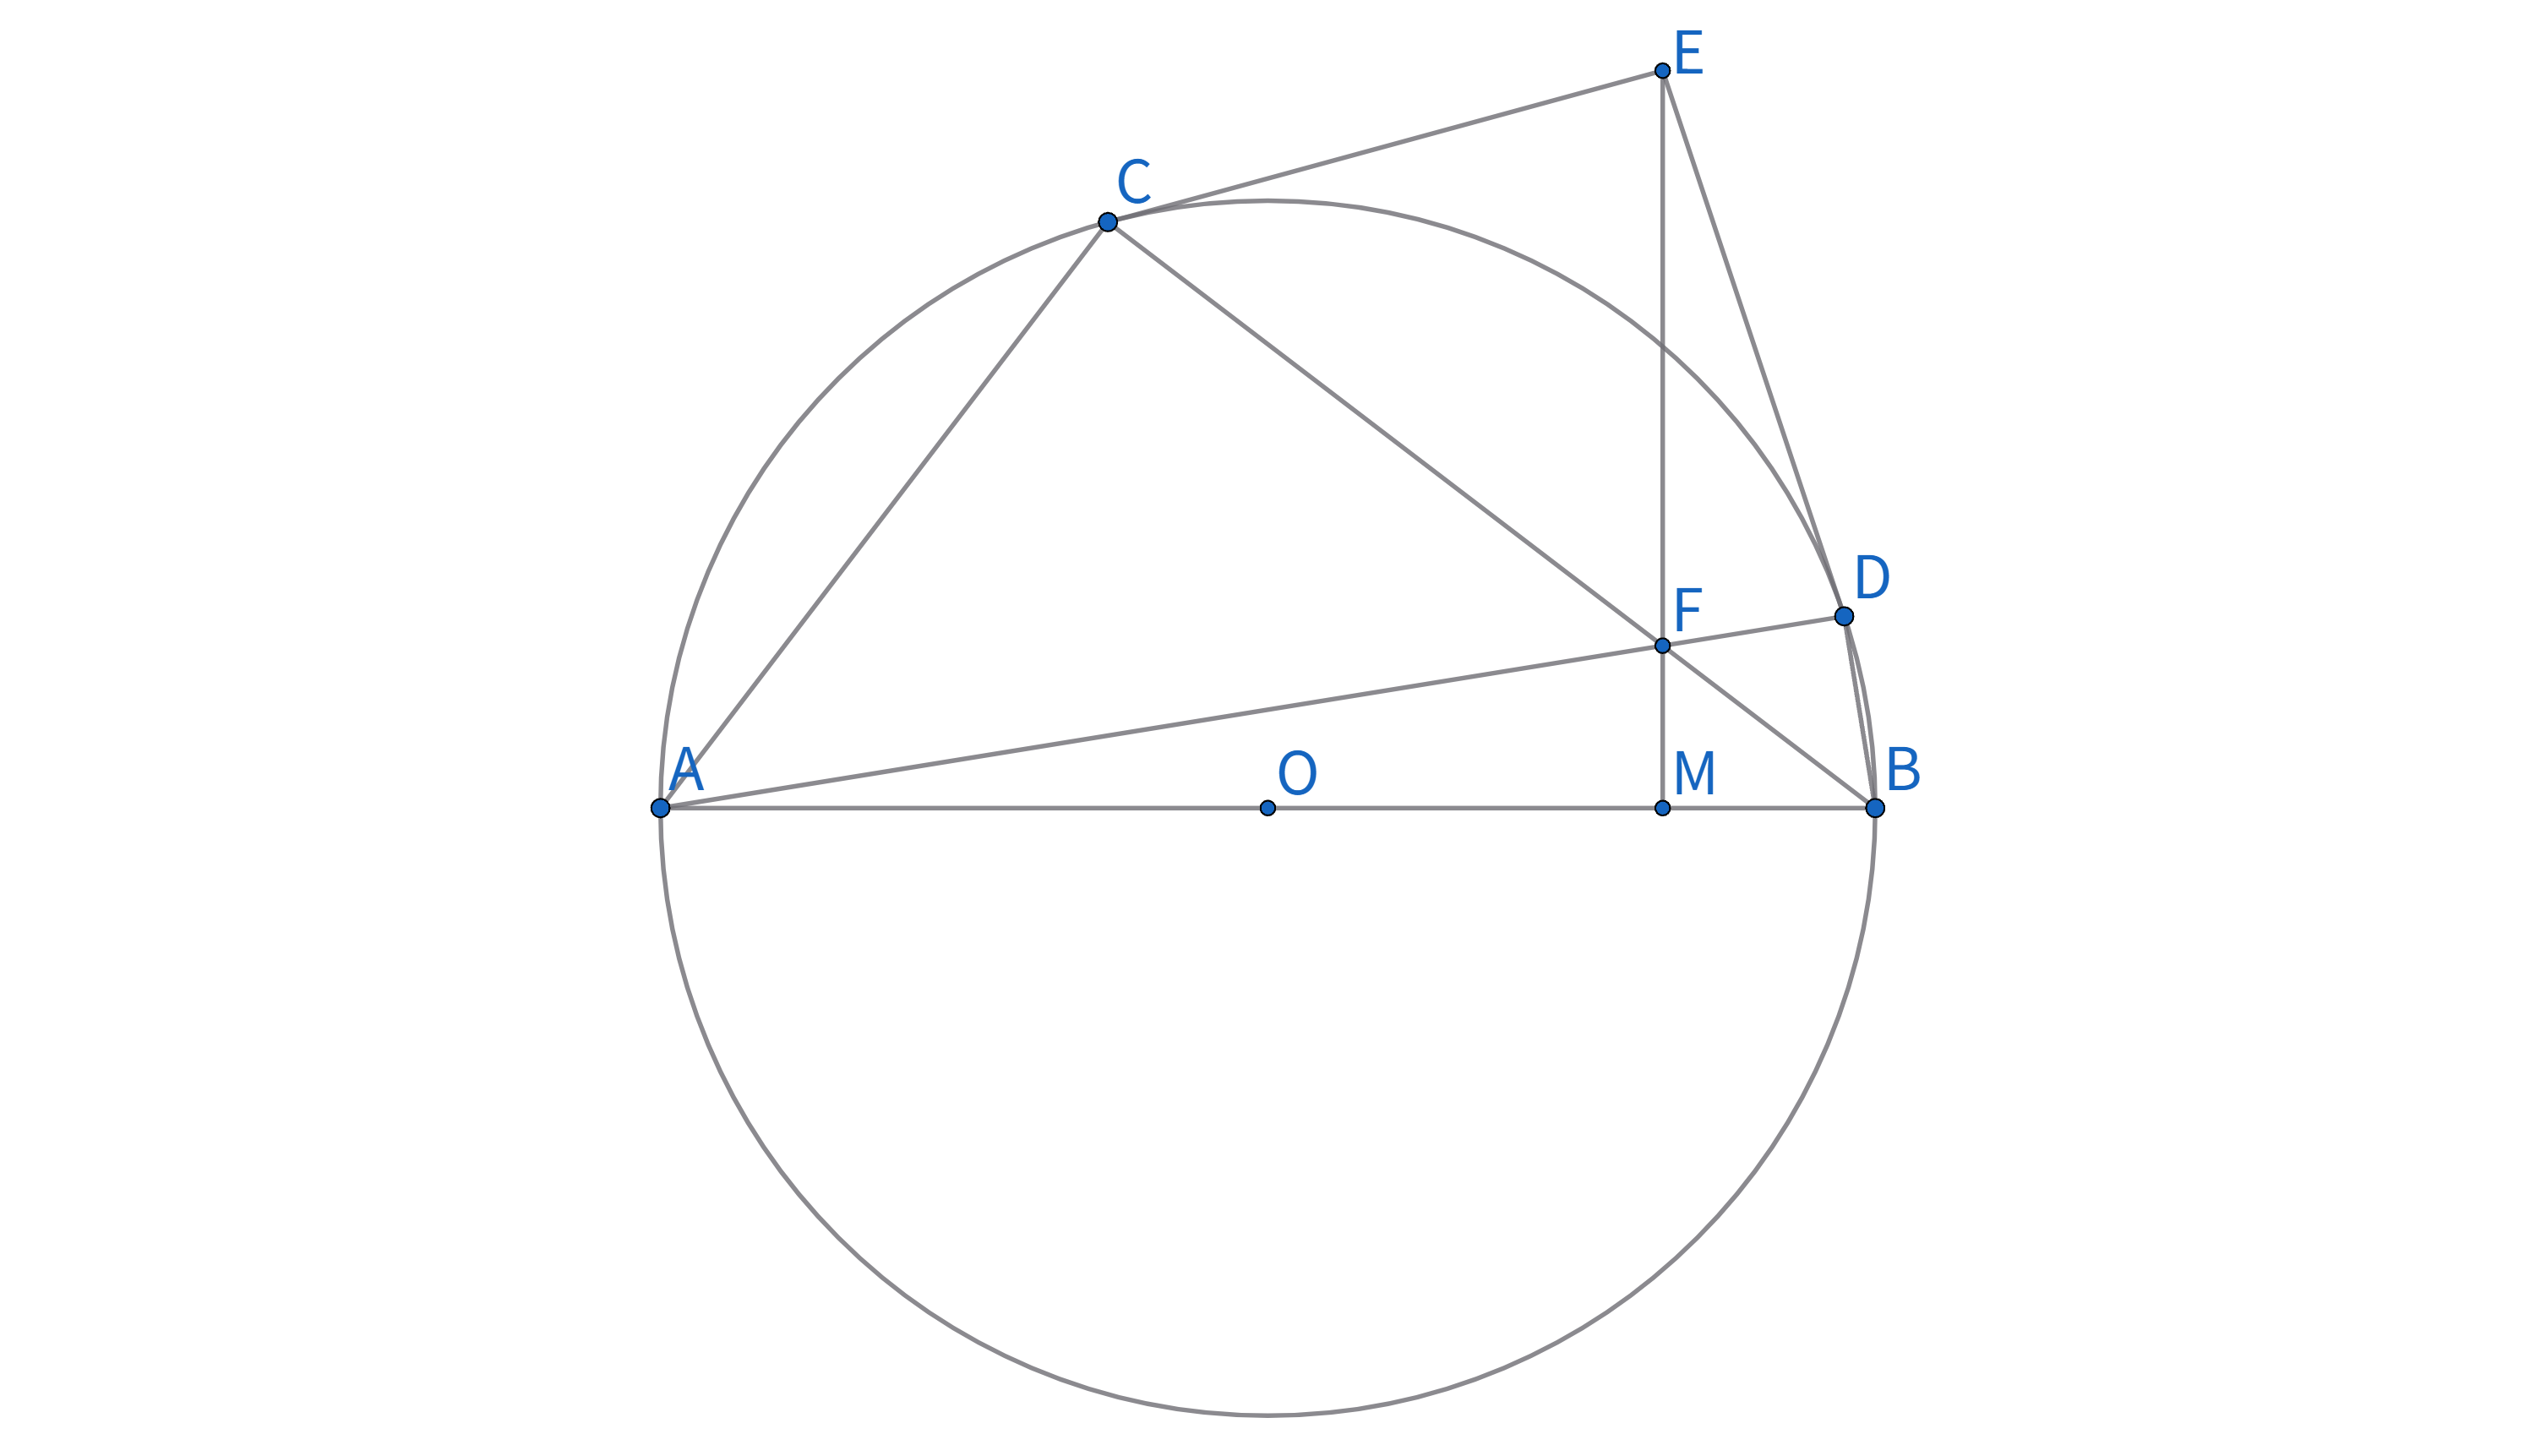
\includegraphics[width=0.8\linewidth]{figures/西部赛10年Q2.png}
\end{figure}

\subsection{Q6}
在 $\triangle ABC$ 中,$\angle ACB = 90^\circ$。以 $B$ 为圆心、$BC$ 为半径作圆,点 $D$ 在边 $AC$ 上,直线 $DE$ 切 $\odot B$ 于点 $E$。过点 $C$ 垂直于 $AB$ 的直线与直线 $BE$ 交于点 $F$,$AF$ 交 $DE$ 于点 $G$,作 $AH \parallel BG$ 交 $DE$ 于点 $H$。求证:$GE = GH$。
\begin{figure}[htbp]
    \centering
    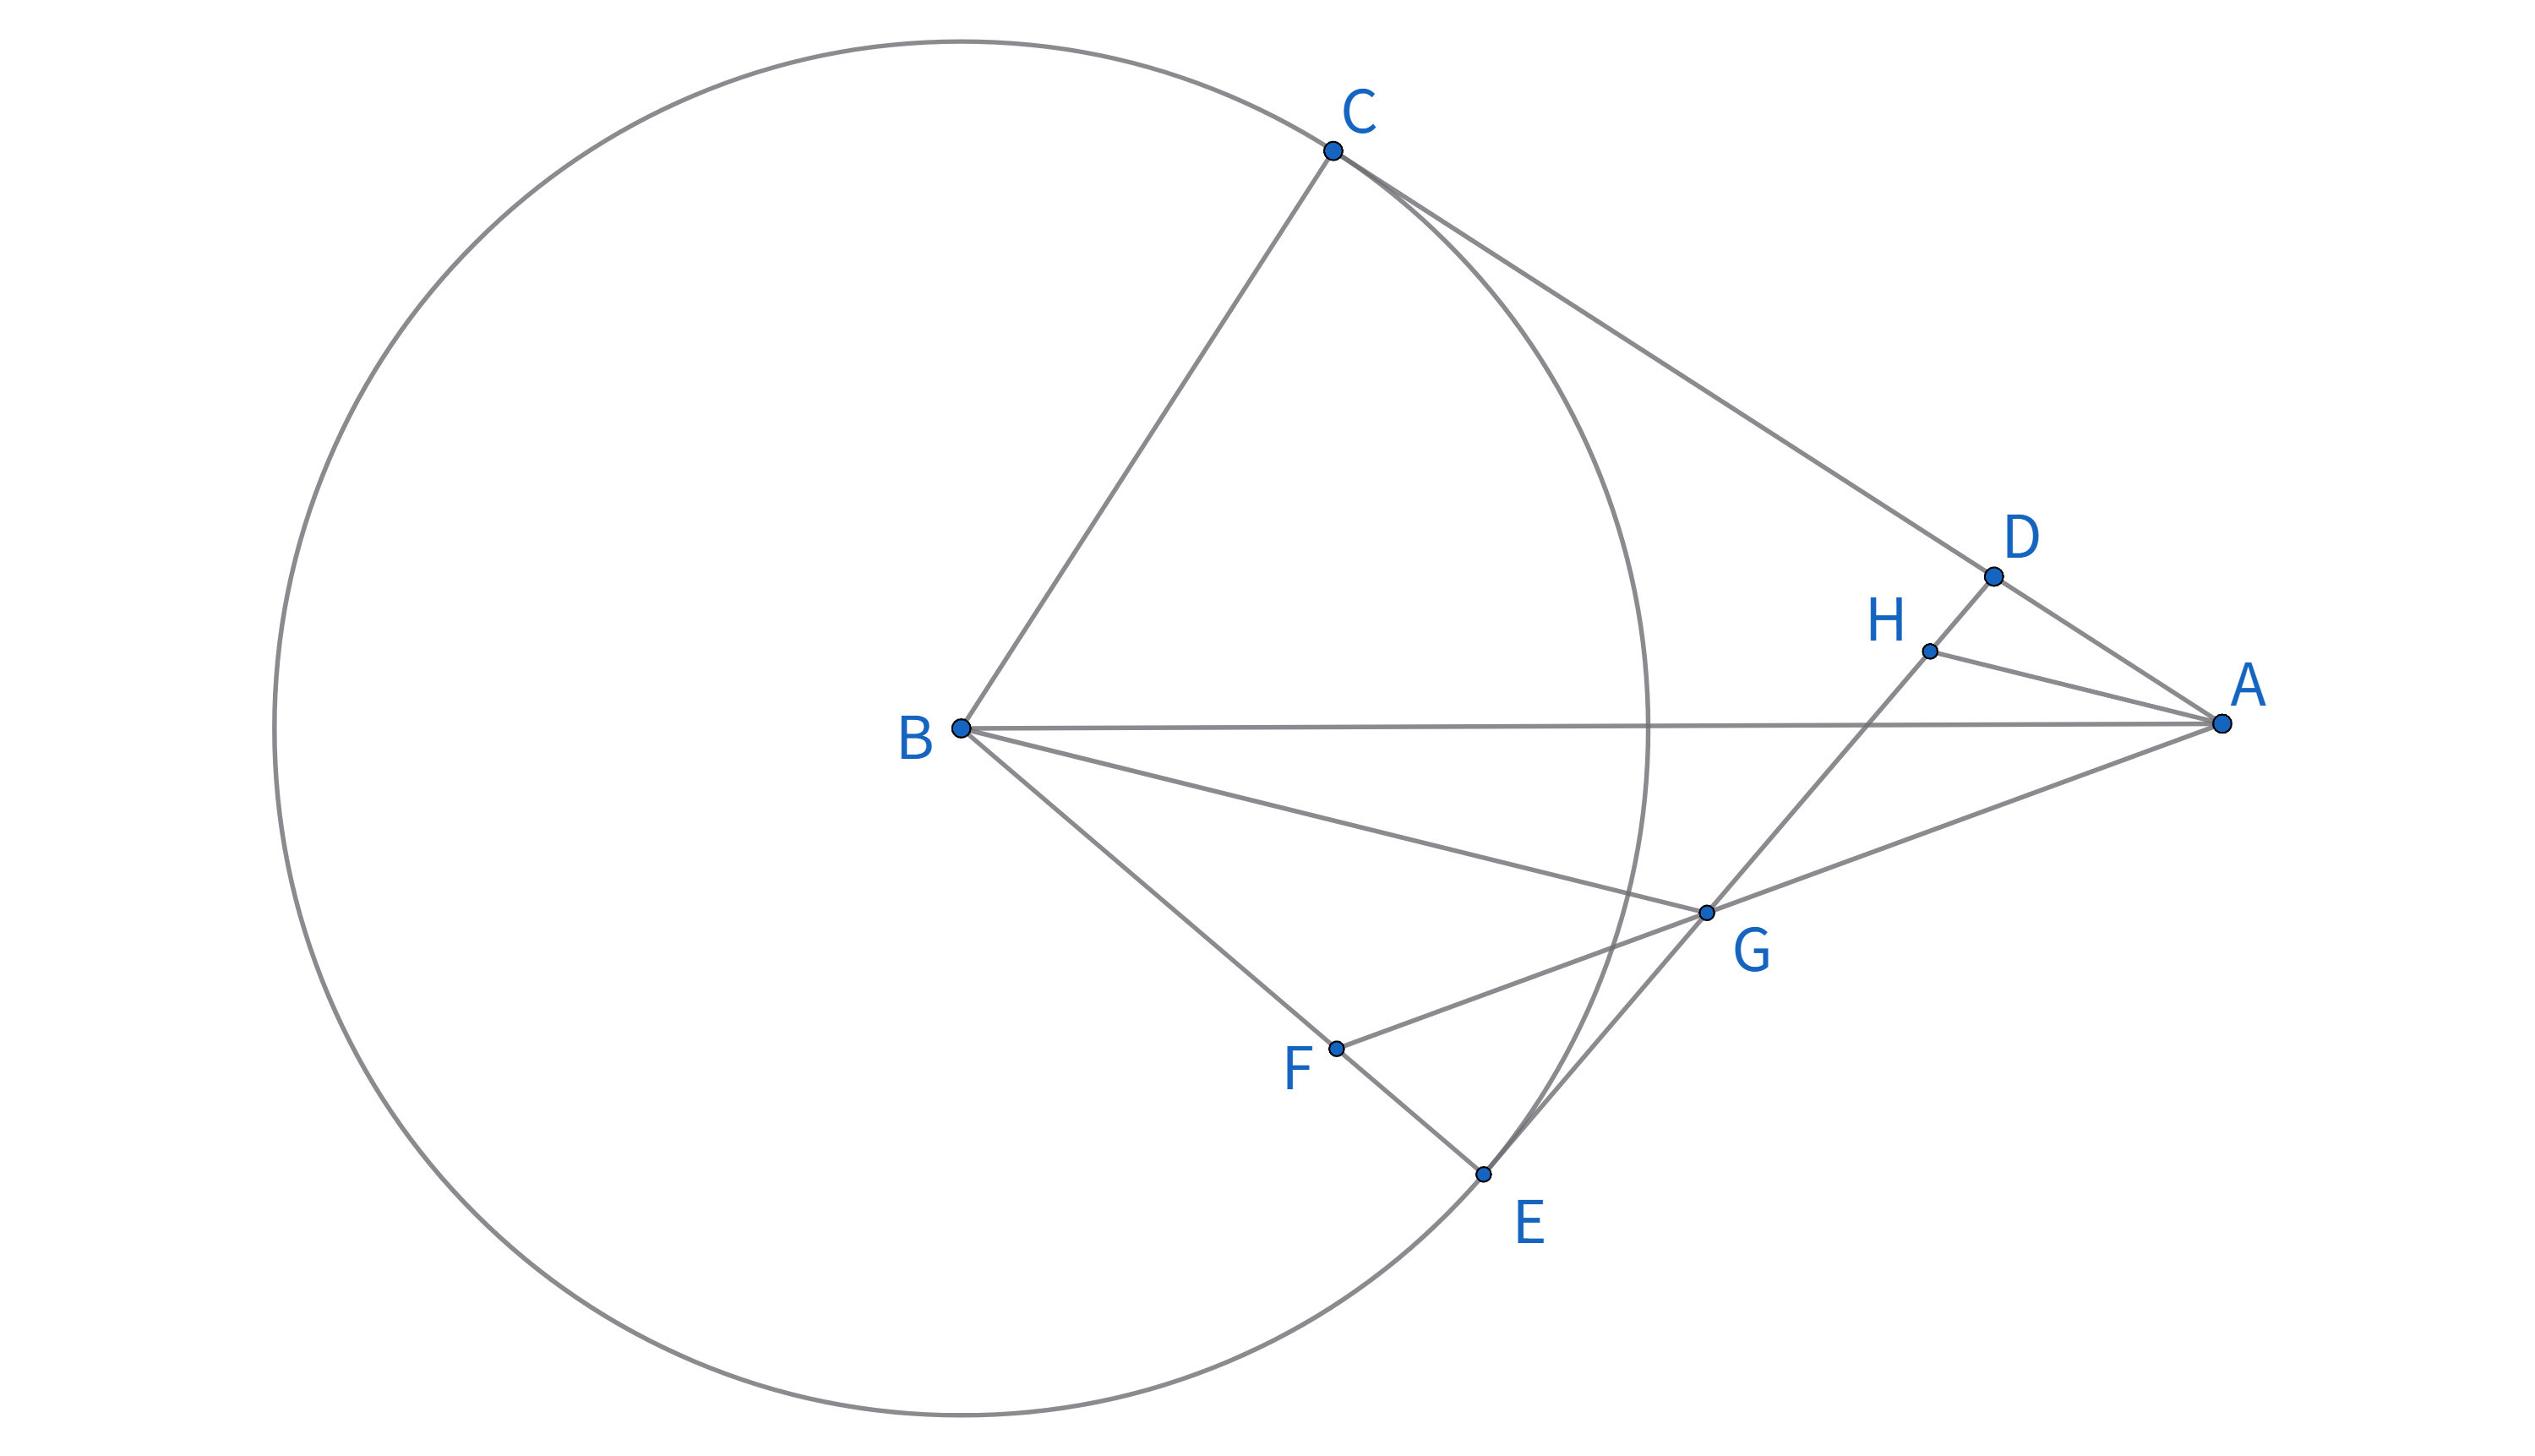
\includegraphics[width=0.8\linewidth]{figures/西部赛10年Q6.png}
\end{figure}


%-------------------------------------------------------------
\newpage
\section{2009年}
\subsection{Q3}
$H$ 为锐角 $\triangle ABC$ 的垂心,$D$ 为边 $BC$ 的中点。过点 $H$ 的直线分别交边 $AB$、$AC$ 于点 $F$、$E$,使得 $AE = AF$。射线 $DH$ 与 $\triangle ABC$ 的外接圆交于点 $P$。求证:$P$、$A$、$E$、$F$ 四点共圆。
\begin{figure}[htbp]
	\centering
	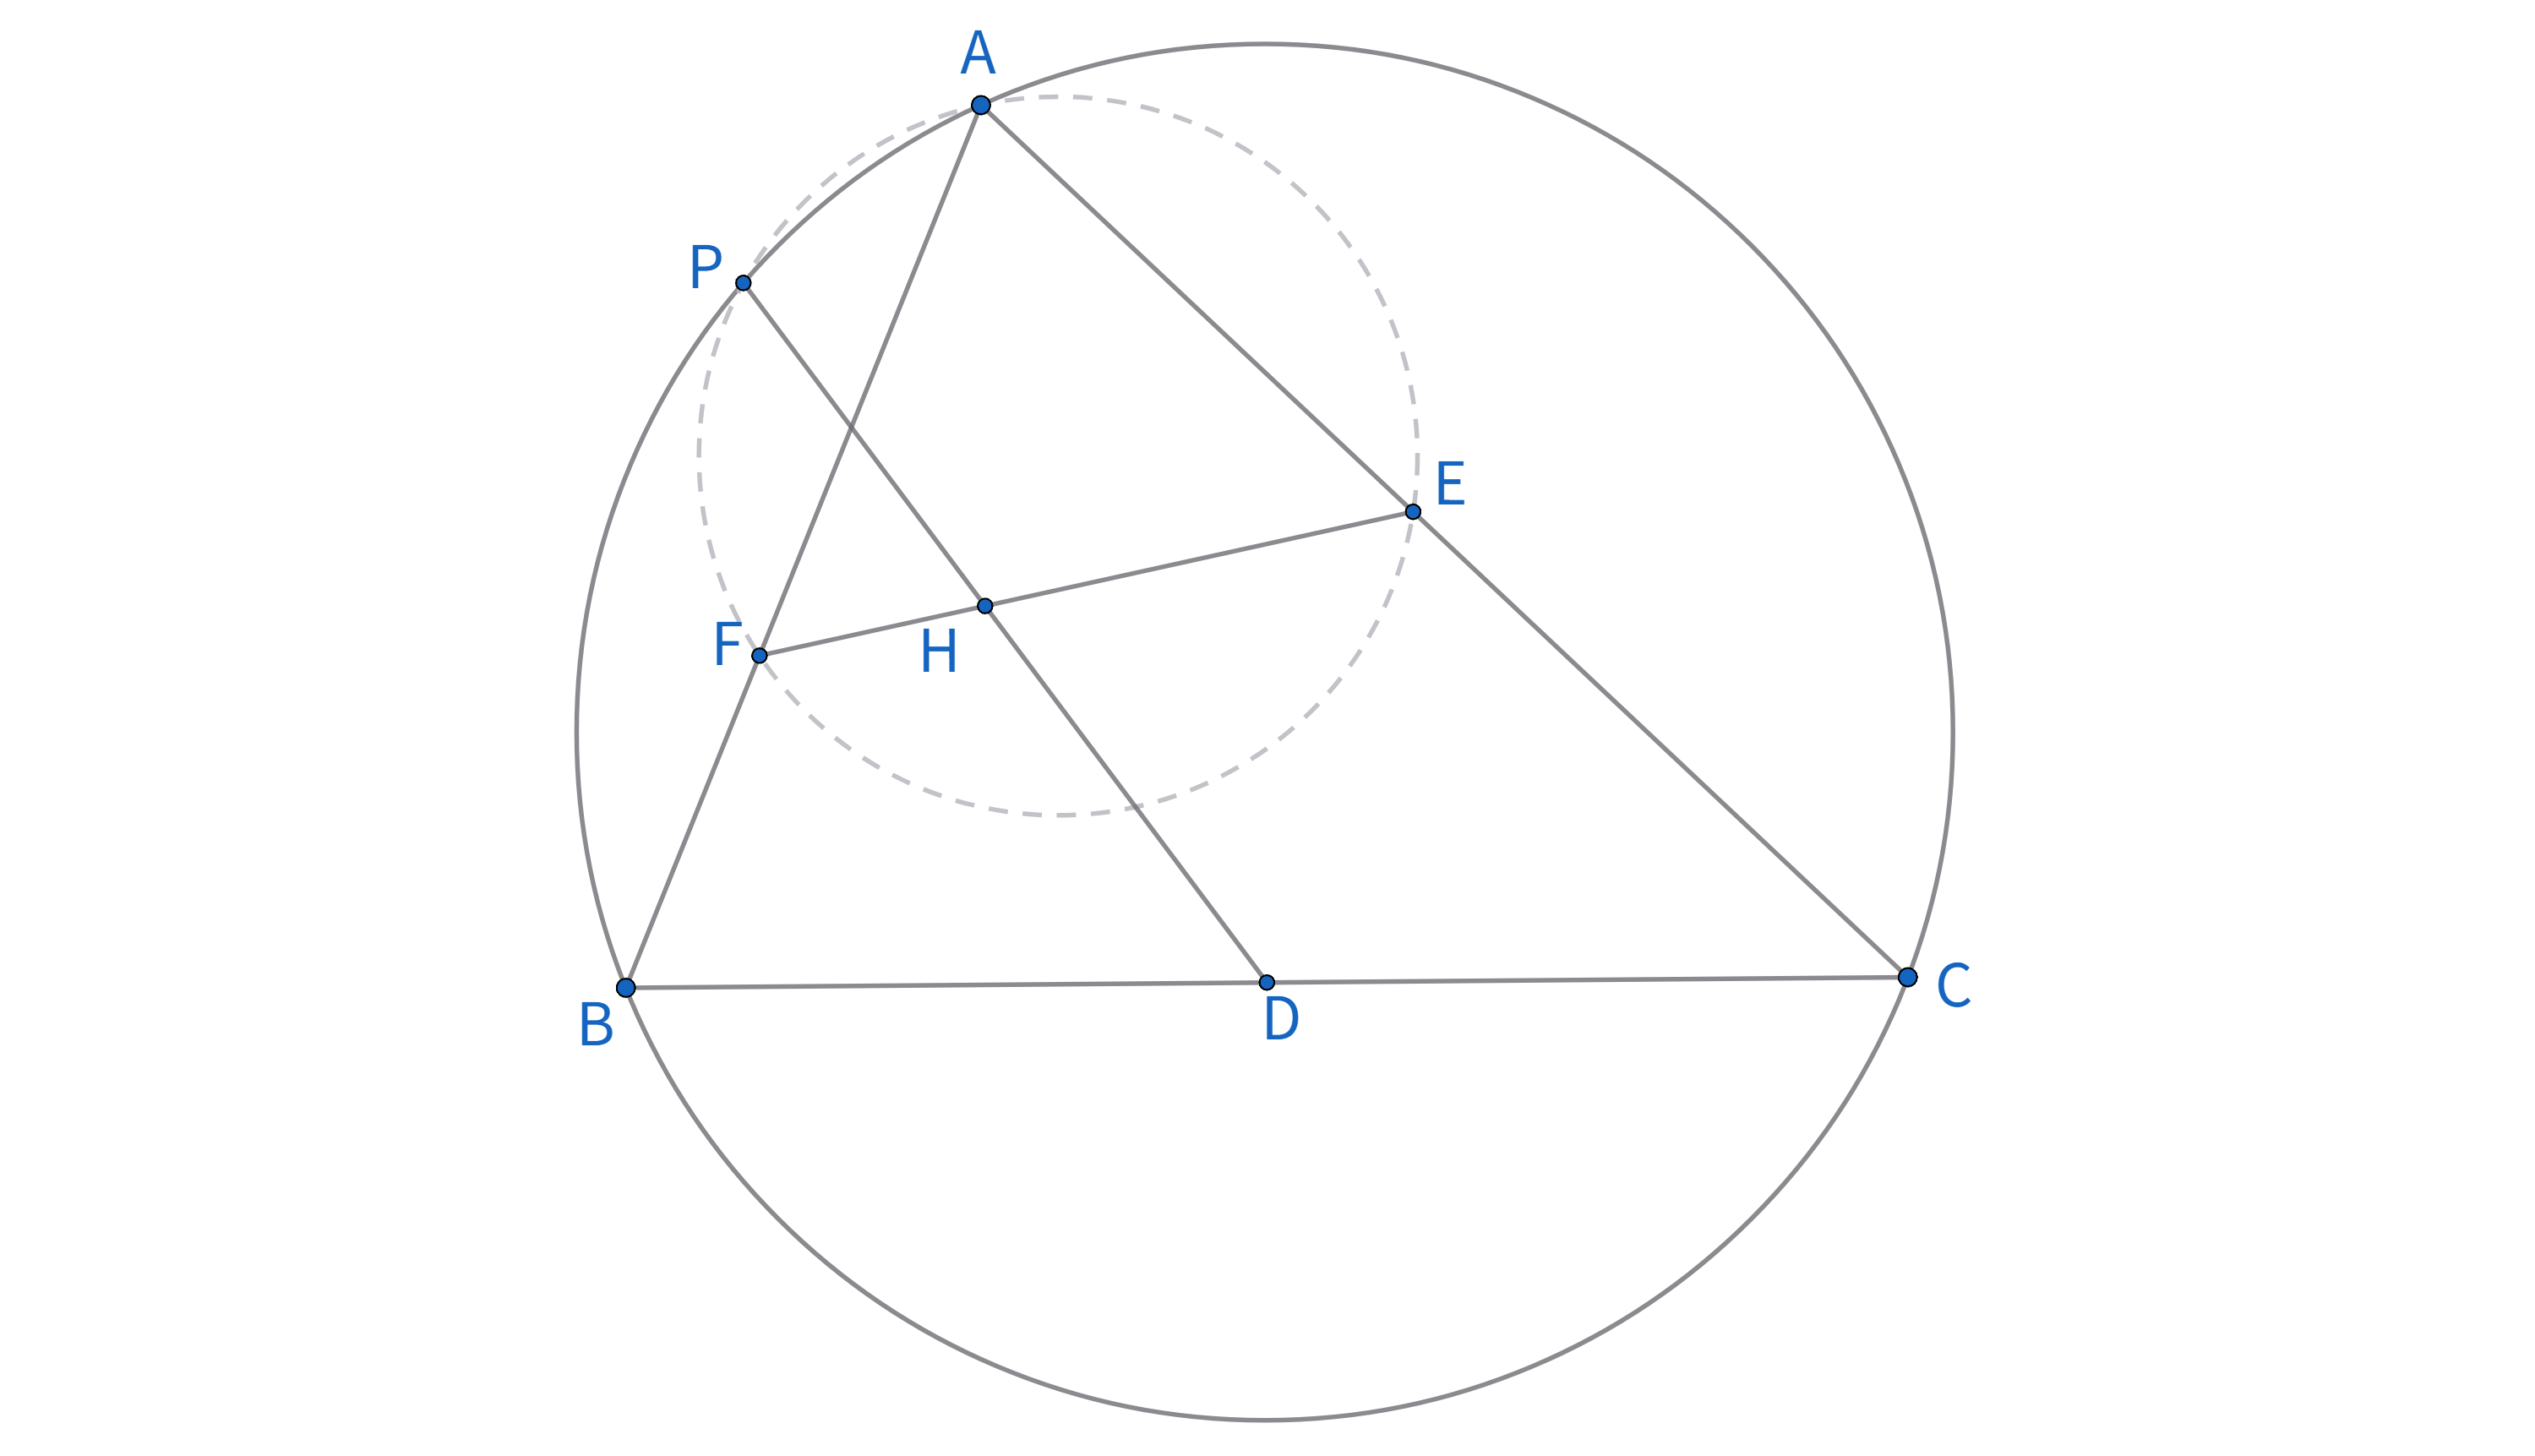
\includegraphics[width=0.8\linewidth]{figures/西部赛09年Q3.png}
\end{figure}

\subsection{Q6}
设点 $D$ 是锐角 $\triangle ABC$ 的边 $BC$ 上一点,以线段 $BD$ 为直径的圆分别交直线 $AB$、$AD$ 于点 $X$、$P$(异于点 $B$、$D$),以线段 $CD$ 为直径的圆分别交直线 $AC$、$AD$ 于点 $Y$、$Q$(异于点 $C$、$D$)。过点 $A$ 作直线 $PX$、$QY$ 的垂线,垂足分别为 $M$、$N$。证明:$\triangle AMN \sim \triangle ABC$ 的充分必要条件是直线 $AD$ 经过 $\triangle ABC$ 的外心。
\begin{figure}[htbp]
	\centering
	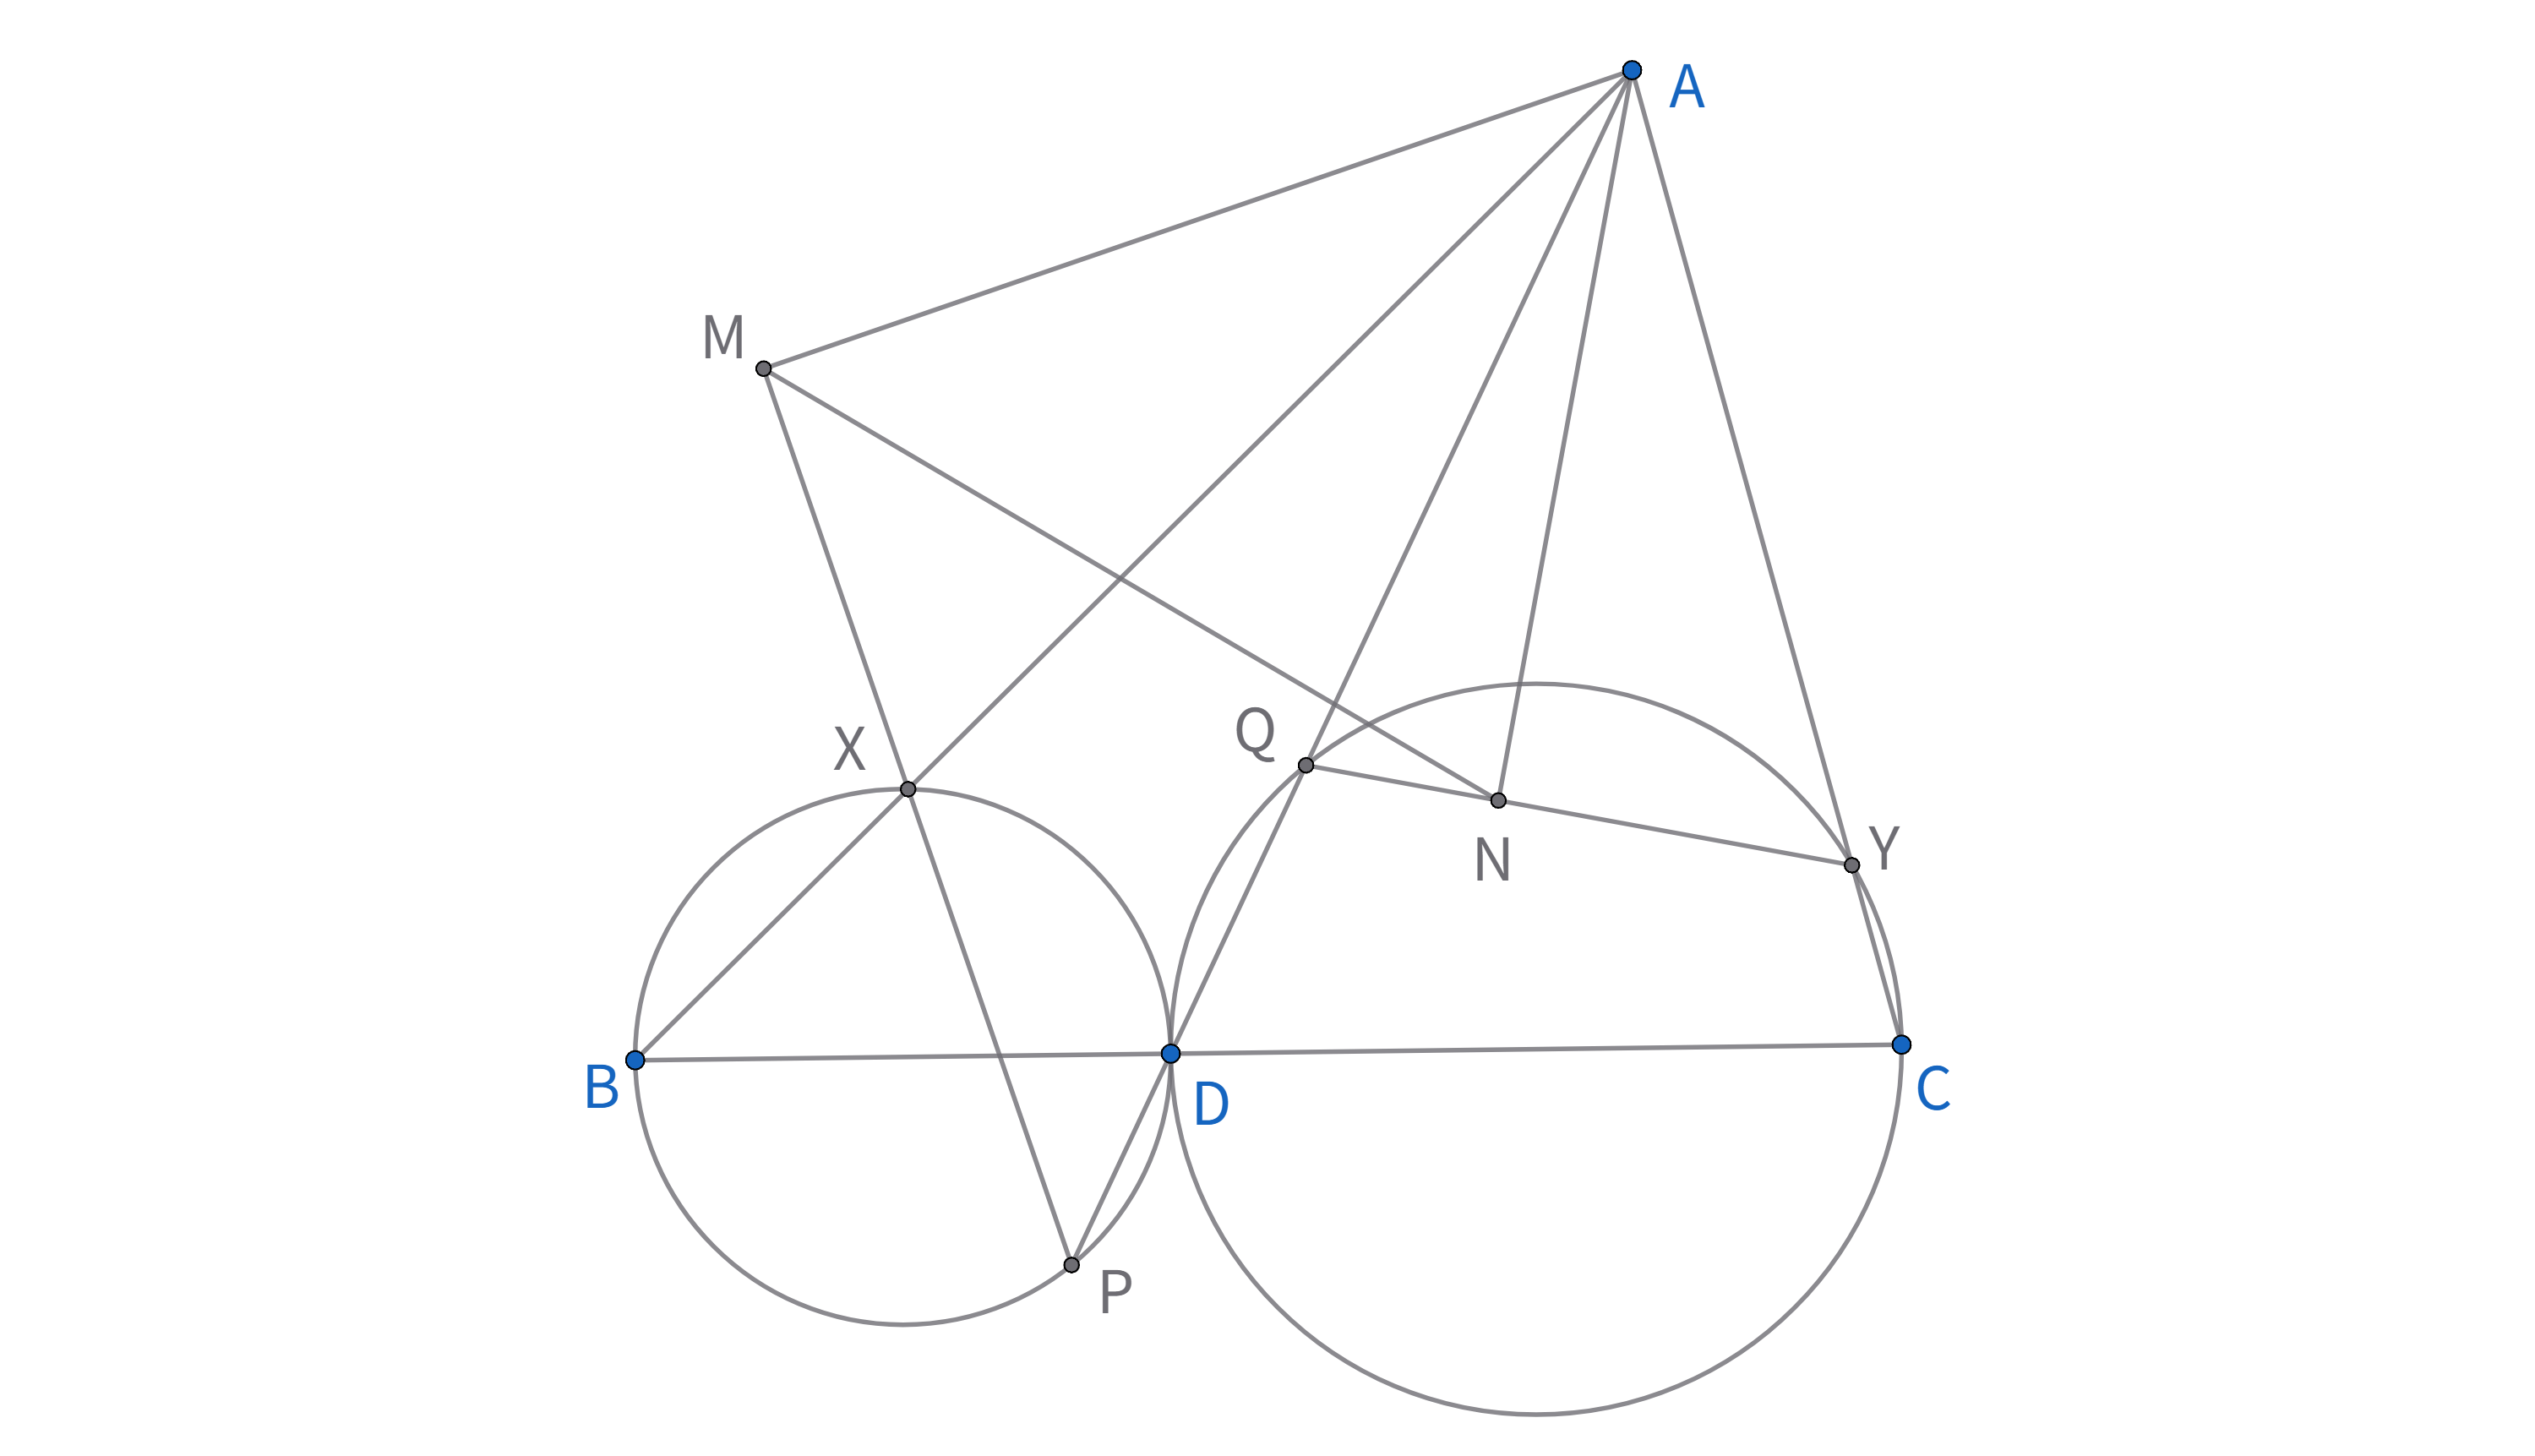
\includegraphics[width=0.8\linewidth]{figures/西部赛09年Q6.png}
\end{figure}




\end{document}